%% NEMA-Q — Quantum Machine Intelligence submission
%% Extended version of ICEQT'26 paper ICE7405.
%% Compile: pdflatex main && bibtex main && pdflatex main && pdflatex main
\documentclass[pdflatex,sn-mathphys-num]{sn-jnl}

\usepackage{graphicx}
\usepackage{multirow}
\usepackage{amsmath,amssymb,amsfonts}
\usepackage{amsthm}
\usepackage{mathrsfs}
\usepackage[title]{appendix}
\usepackage{xcolor}
\usepackage{textcomp}
\usepackage{manyfoot}
\usepackage{booktabs}

\raggedbottom

\begin{document}

\title[Component Accounting in Hybrid Quantum--Classical Graph Learning]{Component Accounting in Hybrid Quantum--Classical Graph Learning: Frozen Circuits Match Trained Ones, and Explainability Shows Why}

\author*[1]{\fnm{MD Nurol} \sur{Amin}}\email{meteormahadi@gmail.com}

\affil*[1]{\orgname{Daffodil International University}, \orgaddress{\city{Dhaka}, \country{Bangladesh}}}

\abstract{Hybrid quantum--classical models are typically evaluated by a single aggregate accuracy number, which cannot say \emph{which} component earned it. We propose component accounting: an evaluation protocol that decomposes a hybrid architecture's performance into per-component contributions using parameter-matched configuration swaps, paired-seed statistics, and gradient telemetry, applied here to NEMA-Q, a hybrid graph network combining a hyperbolic encoder, a variational quantum circuit (PQC), and a classical bypass trunk under gated residual fusion. Across four node-classification datasets stratified by Gromov $\delta$-hyperbolicity (Cora, Citeseer, Pubmed, Disease), the accounting yields findings that a single accuracy column would hide. First, training the quantum circuit never measurably helps: in preregistered confirmatory runs a frozen-random PQC matches or exceeds its trained counterpart in mean on three of four datasets (Cora: $+4.5$ accuracy points, Wilcoxon $p=0.019$, $d=0.87$; marginal under family-wise correction) and is statistically indistinguishable on the fourth; the registered falsifier --- trained significantly better --- is approached nowhere. The value the quantum branch adds, where it adds any, comes from a fixed nonlinear random projection rather than trained quantum features; an exploratory control that rescales the angle embedding to its full range amplifies the effect (frozen better by $+11.8$ points, 10/10 seeds), ruling out the near-identity embedding regime as the artifact behind it. Second, gated fusion fails catastrophically when a branch's compressed input loses per-node signal variance: on Citeseer the quantum branch's angle embedding collapses to near-constant output while contributing the largest gradients in the network, destabilizing training ($0.508\pm0.063$ vs.\ $0.717$ for GCN under the default recipe); per-branch deep supervision restores trunk-level accuracy ($0.638\pm0.019$ confirmatory), and we state a measurable precondition for stable hybrid fusion. Third, the hyperbolic encoder outperforms a parameter-matched Euclidean control in pooled analysis (Stouffer $p=0.040$), but the gains do not track $\delta$-hyperbolicity: the registered negative $\delta$--gain prediction is not observed (weakly positive trend, $\rho=+0.40$ over four datasets) and the gain on the exact-tree dataset is zero --- the standard tree-likeness motivation fails on this suite. The registered low-label quantum-advantage test is likewise null (PQC ahead in mean on all three citation networks, significant on none; pooled $p=0.41$), and a preregistered gate--attribution validity test fails: fusion gates track branch usage, not branch usefulness. Across the completed primary family, no registered hypothesis survives family-wise correction at $\alpha=0.05$ (closest: frozen-vs-trained on Cora, Holm $p=0.056$) --- the paper reports this as the finding rather than burying it. All attribution claims pass through a Quantum Observable Attribution (QOA) faithfulness harness --- masking, perturbation, and model-randomization checks; the single randomization failure (Disease) replicates in confirmatory runs and localizes an input-dominated attribution regime. Code, run manifests, and the frozen preregistration are released.}

\keywords{quantum machine learning, graph neural networks, explainability, hyperbolic geometry, variational quantum circuits, ablation methodology}

\maketitle

\section{Introduction}\label{sec:intro}

A recurring pattern in hybrid quantum--classical machine learning is the composite architecture: a quantum circuit embedded among classical modules, evaluated end-to-end, and reported with a single accuracy number. When such a model performs well, the quantum component absorbs the credit; when it performs poorly, the result is rarely published. Neither outcome tells us what the circuit actually contributed. Recent benchmarking critiques identify exactly this attribution gap --- quantum models compared against untuned classical baselines, under undisclosed budgets, with no isolation of components --- as a dominant methodological bottleneck in the field \cite{qdl2026review,shchur2018pitfalls,huang2021power}.

This paper treats the attribution question as the primary object of study. We take NEMA-Q --- a hybrid graph neural network that fuses a hyperbolic (Poincar\'e-ball) encoder, a variational quantum circuit branch, and a classical GCN bypass through gated residual fusion --- and subject it to \emph{component accounting}: a protocol in which every architectural claim is paired with a control reachable by configuration swap alone, evaluated under paired seeds and identical splits, with per-branch gradient telemetry recorded throughout, and with attribution methods whose own faithfulness is tested rather than assumed.

The accounting produces results that are individually simple but jointly uncomfortable for standard narratives:

\begin{enumerate}
\item \textbf{A frozen-random quantum circuit is never measurably worse than a trained one.} Under an identical scaffold, freezing the PQC's variational parameters at random values matches or exceeds training them in mean on three of four datasets and is indistinguishable on the fourth, significantly so on Cora at the uncorrected level ($+4.5$ points, $p=0.019$, $d=0.87$; marginal under family-wise correction; seeds 10--19, preregistered), and an exploratory full-range-embedding control amplifies the gap to $+11.8$ points in 10/10 seeds. The useful content of the quantum branch, where it exists, is a fixed random nonlinear projection --- the quantum analogue of random-feature methods --- not learned quantum structure.
\item \textbf{Hybrid fusion has a measurable failure precondition.} On Citeseer, the default recipe collapses 21 points below a plain GCN. Telemetry localizes the mechanism: the quantum branch's compressed angle embedding has the lowest input variance of any dataset, producing a branch that is nearly constant across nodes yet injects the largest gradients in the network into shared layers. We state the precondition (per-branch signal variance), show it is measurable before training, demonstrate the repair (per-branch deep supervision), and falsify an alternative explanation.
\item \textbf{The textbook motivation for hyperbolic encoders fails while the encoder itself succeeds.} Hyperbolic beats Euclidean in pooled analysis across the suite, but the registered prediction that gains decrease with Gromov $\delta$ is not observed (the trend is weakly positive over four datasets), the gain on the $\delta=0$ tree is zero, and there a plain GCN beats a dedicated hyperbolic GNN.
\end{enumerate}

None of these findings is visible in an aggregate accuracy table, and the third is invisible without a $\delta$-stratified multi-dataset design. Our contributions, in order of generality: (C1) the component-accounting protocol itself --- configuration-swap controls, paired preregistered statistics, per-branch telemetry --- as a reusable evidentiary standard for hybrid QML; (C2) the frozen-versus-trained control and its outcome, which we argue should become a mandatory baseline for any trained quantum module; (C3) Quantum Observable Attribution with a faithfulness harness that can fail, and once does; (C4) the fusion failure-mode analysis and the branch signal-variance preflight check it yields --- a one-line statistic computable before training.

\paragraph{Relation to the conference version} The ICEQT'26 paper introduced NEMA-Q and Quantum Observable Attribution on Cora only, with five seeds and no tuned baselines. This version answers every methodological objection raised in its review: tuned GCN/GAT/HGCN baselines under identical splits with parameter counts (Sect.~\ref{sec:protocol}); three additional datasets stratified by $\delta$-hyperbolicity (Sect.~\ref{sec:datasets}); a faithfulness validation harness for QOA --- masking, perturbation, and model-randomization checks (Sect.~\ref{sec:qoa}); paired statistical tests with multiple-comparison control for all ablation gaps (Sect.~\ref{sec:stats}); and full reproduction detail via per-run manifests (Sect.~\ref{sec:tuning}). The frozen-vs-trained finding, the fusion failure-mode analysis, and the geometry-mechanism falsification are new.

\section{Related work}\label{sec:related}

\paragraph{Quantum graph learning} Quantum graph neural networks span Hamiltonian-based constructions \cite{verdon2019qgnn}, equivariant circuit families \cite{mernyei2022equivariant}, and recent message-passing formulations analyzed in the Weisfeiler--Leman hierarchy \cite{mpqgnn2026wl}. Most report end-to-end accuracy on small benchmarks; component-level attribution of the quantum contribution is rare. Our architecture is deliberately conservative --- a small angle-embedded circuit with local Pauli-Z readout \cite{benedetti2019pqc,schuld2019feature} --- because the object of study is the accounting, not the circuit.

\paragraph{Random and untrained quantum features} Classically, random feature maps rival trained representations at a fraction of the cost \cite{rahimi2007random}. The quantum counterparts --- quantum reservoir computing and quantum extreme learning machines --- exploit untrained dynamics for information processing \cite{fujii2017qrc,mujal2021qrc,innocenti2023qelm,qelm2025scrambling}. A recent no-free-lunch theorem shows that averaged over tasks, no untrained circuit outperforms any other \cite{herbert2023nfl}. Our H5 result is complementary and sharper in one direction: for a \emph{specific} trained architecture on \emph{specific} tasks, training the circuit is empirically never better and sometimes reliably worse than freezing it --- a statement about optimization in situ, not about task-averaged expressivity. Trainability obstructions offer a mechanism: barren plateaus and related landscape pathologies \cite{mcclean2018barren,cerezo2021cost,holmes2022expressibility,larocca2025barren}, compounded in our setting by an angle-embedding regime that concentrates inputs near zero rotation (Sect.~\ref{sec:failure}).

\paragraph{Dequantization and classical surrogates} Trained PQC models can often be replaced by efficient classical surrogates \cite{tang2019dequant,schreiber2023surrogates,sweke2025rff,shin2024tensor}, and some circuit families are classically simulable outright \cite{qcnn2024simulable}. Our surrogate control (NEMA-C) sits in this lineage: a parameter-matched classical branch substituted for the PQC. Component accounting extends the surrogate question from ``can the quantum model be replaced after training?'' to ``which architectural slot, if any, did quantumness fill during training?''

\paragraph{Hyperbolic graph learning} Poincar\'e embeddings \cite{nickel2017poincare} and hyperbolic GNNs \cite{chami2019hgcn,liu2019hgnn,ganea2018hnn} motivate negative curvature by the tree-like, scale-free structure of real graphs, standardly quantified by Gromov $\delta$-hyperbolicity \cite{adcock2013tree,yang2022hgnnreview}. Recent critical work finds that hyperbolic gains track geometry--task alignment rather than raw structural tree-likeness \cite{alignment2026hyperbolic}; our $\delta$-stratified falsification (Sect.~\ref{sec:geometry}) provides independent, preregistered evidence for that revisionist view.

\paragraph{Explainability for quantum models} Quantum XAI is nascent: Shapley values over circuit gates \cite{heese2025shapley}, classical feature-importance adaptations \cite{qfi2024feature}, representation-level frameworks \cite{qrlaxai2025}, and a general treatment of what explaining QML can and cannot mean \cite{gilfuster2024explaining}. Quantum Observable Attribution differs in target: it attributes a \emph{hybrid} model's per-node decisions to the measured observables at the quantum--classical interface --- the boundary where quantum information becomes classical feature --- rather than to gates or input features. Crucially, we subject QOA to the sanity-check discipline developed for classical saliency \cite{adebayo2018sanity,hooker2019roar} and adopted by the graph-XAI evaluation literature \cite{agarwal2023graphxai,ginxeval2023,robustfidelity2023}, which no prior quantum attribution work has done.

\section{Architecture}\label{sec:arch}

NEMA-Q is a three-branch node classifier (Fig.~\ref{fig:arch}). Given a graph $G=(V,E)$ with node features $x_i \in \mathbb{R}^F$, every branch $b$ maps $(X, E)$ to a node embedding $h_{b,i} \in \mathbb{R}^{e}$ of shared width $e=64$; ablations are configuration swaps, never code forks. We describe each branch, the fusion rule, and the training objective in the exact form implemented; every symbol below corresponds to a named tensor in the released code.

\begin{figure}[t]
\centering
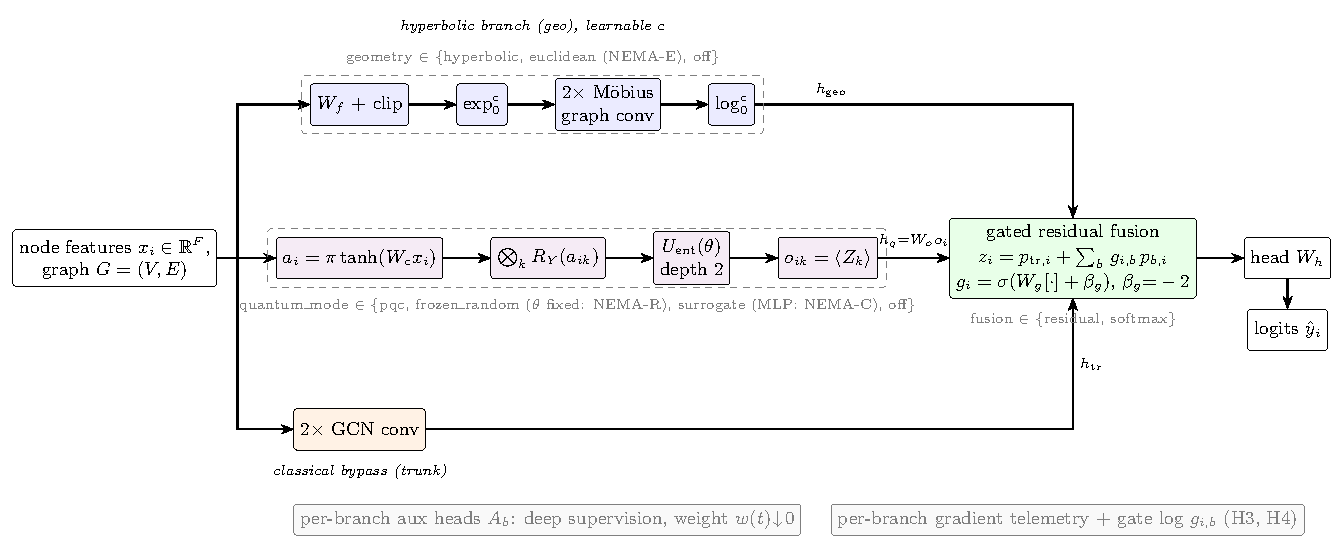
\includegraphics[width=\textwidth]{figs/fig1_architecture.pdf}
\caption{NEMA-Q architecture. Three parallel branches --- hyperbolic encoder (geo), variational quantum circuit (q), and classical GCN bypass (trunk) --- map node features to width-$e$ embeddings. The bypass is the trunk of a gated residual fusion; geo and q enter through sigmoid gates initialized nearly closed ($\sigma(-2)\approx0.12$). Dashed boxes mark the configuration swaps that generate every control in the paper: geometry $\in$ \{hyperbolic, euclidean, off\}, quantum mode $\in$ \{pqc, frozen\_random, surrogate, off\}, fusion $\in$ \{residual, softmax\}. Per-branch auxiliary heads (deep supervision) and per-branch gradient telemetry taps are shown in gray.}
\label{fig:arch}
\end{figure}

\paragraph{Hyperbolic branch (geo)} An HGCN-style encoder on the Poincar\'e ball $\mathbb{B}^e_c = \{u \in \mathbb{R}^e : c\|u\|^2 < 1\}$ with learnable curvature $c$. Exponential and logarithmic maps at the origin,
\begin{equation}
\exp_0^c(v) = \tanh(\sqrt{c}\,\|v\|)\,\frac{v}{\sqrt{c}\,\|v\|}, \qquad
\log_0^c(u) = \operatorname{artanh}(\sqrt{c}\,\|u\|)\,\frac{u}{\sqrt{c}\,\|u\|},
\end{equation}
carry vectors between the ball and its tangent space at the origin. Raw features are first compressed Euclideanly, $t_i = \mathrm{clip}_{2.5}(W_f x_i)$, with tangent norms clipped at $2.5$ before the exp-map --- mapping high-dimensional sparse features (e.g.\ Cora's 1433-dimensional bags-of-words) directly onto the ball saturates points at the boundary where gradients vanish. Each of two graph-convolution layers then applies a M\"obius linear transform followed by tangent-space aggregation:
\begin{equation}
u_i = (W \otimes_c h_i) \oplus_c \exp_0^c(\beta), \qquad
h'_i = \exp_0^c\!\Big(\phi\Big(\tfrac{1}{|\mathcal{N}(i)|+1}\textstyle\sum_{j \in \mathcal{N}(i)\cup\{i\}} \log_0^c(u_j)\Big)\Big),
\end{equation}
where $\otimes_c$ and $\oplus_c$ are M\"obius matrix--vector product and addition \cite{ganea2018hnn}, and $\phi$ is ReLU + dropout (identity in the final layer). The branch output is $\log_0^c$-mapped so fusion operates in a shared tangent space. Curvature $c$ is a learnable (positivity-constrained) parameter; its learned per-dataset value is itself reportable evidence for H1. The \texttt{euclidean} swap replaces the entire branch with a width-matched GCN encoder (control NEMA-E); \texttt{off} removes it.

\paragraph{Quantum branch (q)} A classical compressor maps features to $n=4$ bounded rotation angles,
\begin{equation}
a_i = \pi \tanh(W_c x_i + \beta_c) \in [-\pi, \pi]^n,
\end{equation}
which enter a depth-$L$ ($L=2$) strongly-entangling circuit \cite{schuld2019feature} via single-qubit $R_Y$ rotations:
\begin{equation}
|\psi_i(\theta)\rangle = U_{\text{ent}}(\theta)\,\Big(\textstyle\bigotimes_{k=1}^{n} R_Y(a_{ik})\Big)\,|0\rangle^{\otimes n},
\end{equation}
with $U_{\text{ent}}$ the StronglyEntanglingLayers ansatz (per-layer general single-qubit rotations plus a ring of CNOTs; $|\theta| = 3nL$). The branch reads out the $n$ local Pauli-Z expectations and projects them to the branch width:
\begin{equation}
o_{ik} = \langle \psi_i(\theta) | Z_k | \psi_i(\theta) \rangle, \qquad
h_{q,i} = W_o\, o_i + \beta_o.
\end{equation}
Figure~\ref{fig:circuit} shows the compiled circuit. The observable vector $o_i$ is the quantum--classical boundary that QOA attributes against (Sect.~\ref{sec:qoa}).

\begin{figure}[t]
\centering
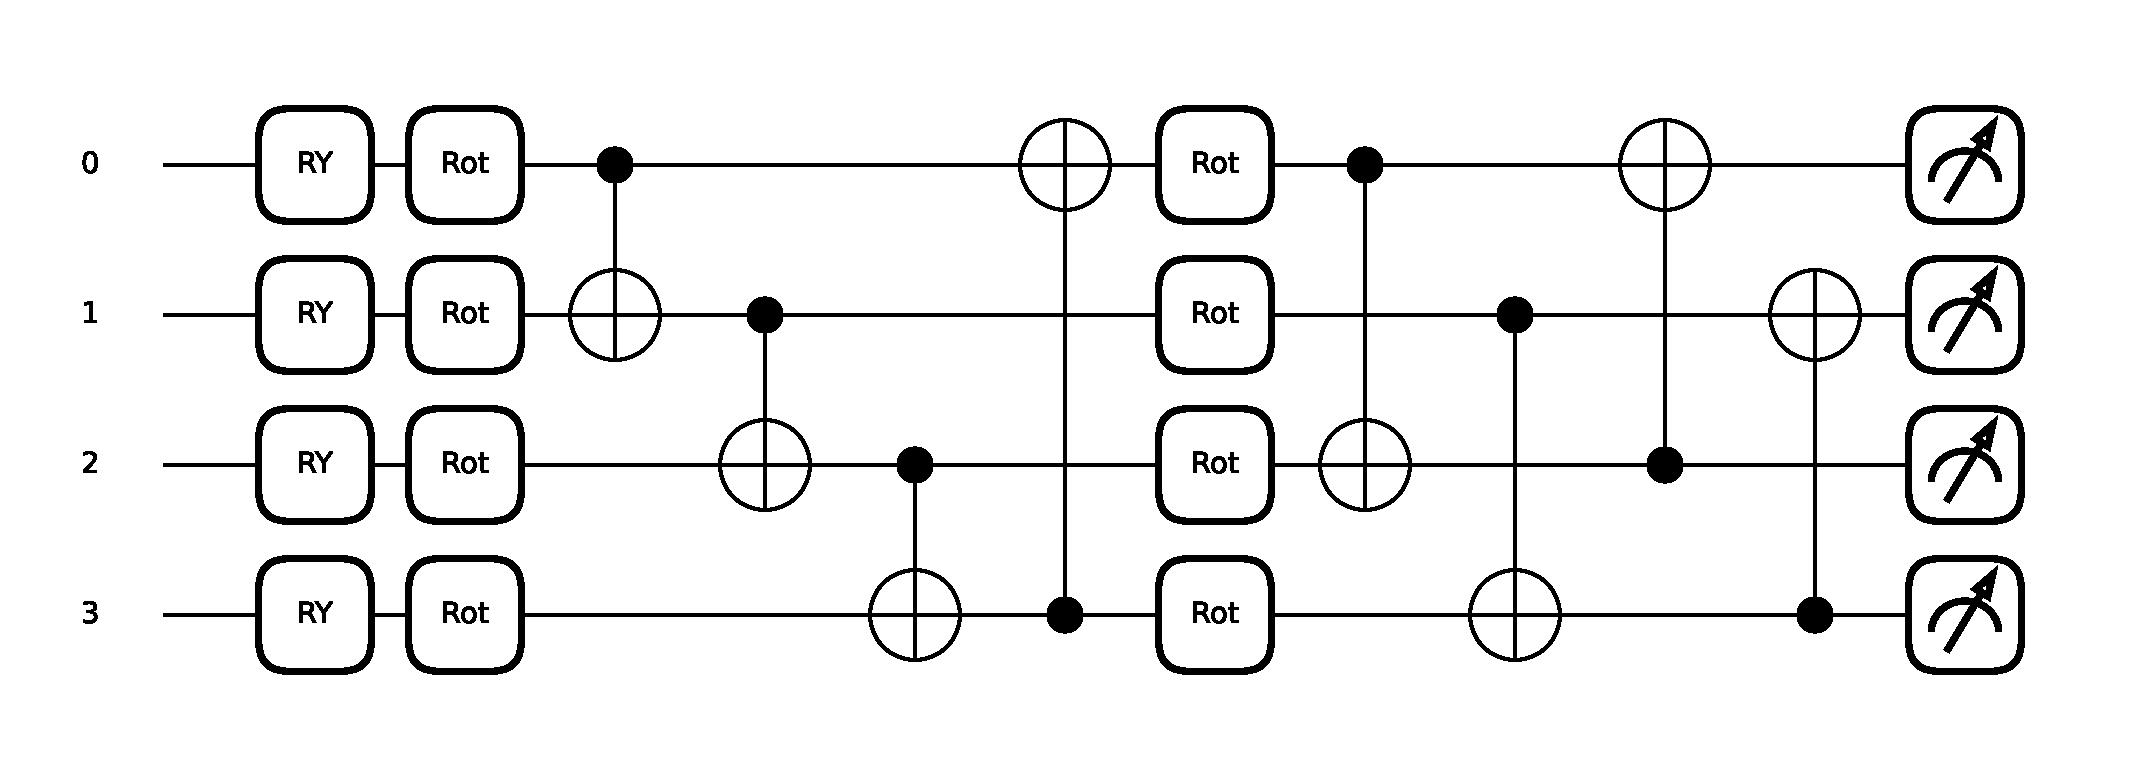
\includegraphics[width=\textwidth]{figs/quantum_circuit.pdf}
\caption{The quantum branch's circuit, compiled to device gates ($n=4$ qubits, depth $L=2$). Per-qubit $R_Y$ gates realize the angle embedding of the compressed inputs $a_{ik}$; each StronglyEntanglingLayers block applies one general single-qubit rotation $\mathrm{Rot}(\theta) = R_Z R_Y R_Z$ per qubit followed by a CNOT ring (nearest-neighbor in the first layer, range-2 in the second), for $|\theta| = 3nL = 24$ trainable parameters; readout is the four local Pauli-Z expectations $\langle Z_k \rangle$. NEMA-R freezes exactly these 24 parameters at seeded random values.}
\label{fig:circuit}
\end{figure} Swaps: \texttt{frozen\_random} --- identical circuit with $\theta \sim \mathcal{U}[0, 2\pi)^{|\theta|}$ drawn once from a fixed seed and excluded from the optimizer (control NEMA-R); \texttt{surrogate} --- parameter-matched classical MLP (NEMA-C); \texttt{off}. The circuit is deliberately small, with $n \le 8$, $L \le 4$ enforced as assertions in code, to stay inside barren-plateau safe budgets \cite{larocca2025barren}; exact statevector simulation is used throughout, with finite-shot execution as a preregistered ablation.

\paragraph{Classical bypass (trunk)} A plain two-layer GCN encoder \cite{kipf2017gcn} producing $h_{\text{tr},i}$.

\paragraph{Gated residual fusion} Each branch is projected to the fused width $d=64$, $p_{b,i} = W_b h_{b,i}$, and the non-trunk branches enter as sigmoid-gated residuals on the trunk:
\begin{equation}
g_i = \sigma\big(W_g\,[\,p_{b_1,i}; \dots ; p_{b_B,i}\,] + \beta_g\big) \in (0,1)^{B-1}, \qquad
z_i = p_{\text{tr},i} + \textstyle\sum_{b \ne \text{tr}} g_{i,b}\; p_{b,i},
\end{equation}
with $W_g$ zero-initialized and $\beta_g$ initialized at $-2$ ($\sigma(-2)\approx0.12$), so training starts from ``approximately a GCN'' and exotic branches must earn gate mass. This is the graceful-degradation guarantee --- tested, and on one dataset broken and repaired, in Sect.~\ref{sec:failure}; the initialization is exposed as the config knob \texttt{gate\_bias\_init} that the repair tunes. Per-node gate values $g_{i,b}$ are recorded for telemetry and H4. The \texttt{softmax} fusion swap replaces the rule with all-branch competition, $g_i = \mathrm{softmax}(W_g[\cdot] + \beta_g) \in \Delta^{B-1}$, $z_i = \sum_b g_{i,b}\,p_{b,i}$ --- retained as the instability ablation (Sect.~\ref{sec:fusion}). Class logits are $\hat{y}_i = W_h z_i$.

\paragraph{Deep supervision} Each branch carries an auxiliary linear classifier $A_b$ trained against the labels; the total objective on the training mask is
\begin{equation}
\mathcal{L} = \mathrm{CE}(\hat{y}, y) + w(t)\,\frac{1}{B}\sum_{b} \mathrm{CE}(A_b h_{b}, y), \qquad
w(t) = \lambda_{\text{aux}}\Big(1 - \frac{t}{T}\Big),
\end{equation}
with the auxiliary weight annealed linearly to zero over the $T$ training epochs: early anti-starvation \cite{lee2015deeply} without late-training interference. Section~\ref{sec:failure} quantifies why this term is load-bearing --- $\lambda_{\text{aux}}$ is the single knob that repairs the Citeseer collapse.

Parameter matching between the PQC and surrogate branches is enforced by test at 15\% tolerance; per-branch and total counts are recorded in every run manifest (Appendix~\ref{app:params}).

\section{Experimental protocol}\label{sec:protocol}

\subsection{Datasets and \texorpdfstring{$\delta$}{delta}-stratification}\label{sec:datasets}

We evaluate on Cora, Citeseer, Pubmed (Planetoid public splits \cite{yang2016planetoid}) and Disease \cite{chami2019hgcn} (synthetic SIR tree; stratified 30/10/60 split, no public split exists). Sampled four-point Gromov $\delta$ on the largest component stratifies the suite (Table~\ref{tab:datasets}): Disease $\delta=0.000$ is the exact tree --- the positive control where hyperbolic geometry must help if the tree-likeness mechanism is real --- with Cora, Pubmed, and Citeseer progressively less hyperbolic. The suite simultaneously spans two potential confounders that Sect.~\ref{sec:failure} will need: feature density varies by two orders of magnitude ($0.009$--$1.0$) and largest-component fraction from $0.64$ to $1.0$.

\begin{table}[t]
\centering
\caption{Dataset suite, $\delta$-stratified. $\delta$ is sampled four-point Gromov hyperbolicity on the largest connected component; homophily is edge homophily; density is feature density (fraction of nonzero feature entries).}
\label{tab:datasets}
\footnotesize
\begin{tabular}{@{}lrrrrrrrrr@{}}
\toprule
Dataset & Nodes & Edges & Feat. & Cls. & $\delta_{\text{mean}}$ & $\delta_{\max}$ & Homoph. & Density & LCC \\
\midrule
Disease  & 1{,}044  & 1{,}043  & 1{,}000 & 2 & 0.000 & 0.0 & 0.875 & 1.000 & 1.00 \\
Cora     & 2{,}708  & 5{,}278  & 1{,}433 & 7 & 0.356 & 2.0 & 0.810 & 0.013 & 0.92 \\
Pubmed   & 19{,}717 & 44{,}324 & 500     & 3 & 0.399 & 3.5 & 0.802 & 0.100 & 1.00 \\
Citeseer & 3{,}327  & 4{,}552  & 3{,}703 & 6 & 0.550 & 3.5 & 0.736 & 0.009 & 0.64 \\
\bottomrule
\end{tabular}
\end{table}

\subsection{Hypotheses}\label{sec:hypotheses}

Preregistered before the confirmatory runs (repository commit \texttt{4605c73}, frozen 2026-07-17):

\begin{itemize}
\item \textbf{H1 (geometry, two-part).} (a) Direction: hyperbolic $>$ parameter-matched Euclidean (NEMA-Q vs.\ NEMA-E), pooled across datasets by Stouffer's $Z$ over per-dataset one-sided Wilcoxon tests. The pooled test is primary because the conference pilot showed single-dataset comparisons are underpowered at $n=10$ seeds (Cora paired $d=0.44$ implies ${\sim}40$ seeds for 80\% power alone). (b) Mechanism: paired gain decreases with $\delta$ (Spearman over datasets). Part (b) is the standard literature claim; we register both so that either can fail independently. \emph{Falsifiers:} pooled $p \ge 0.05$ (a); no negative $\delta$--gain correlation (b).
\item \textbf{H2 (quantum vs.\ surrogate).} NEMA-Q $>$ NEMA-C at $\le 5$ labels per class, with the gap closing at standard label rates; paired Wilcoxon per (dataset, label rate). \emph{Falsifier:} surrogate matches the PQC at all label rates.
\item \textbf{H3 (trainability telemetry).} PQC circuit-weight gradient variance stays within two orders of magnitude of the best classical branch's gradient variance on $\ge 9/10$ seeds --- a relative criterion, because absolute barren-plateau floors from the literature do not transfer to a trained hybrid; the classical branches are the matched healthy-gradient reference at the same loss scale. \emph{Falsifier:} sustained relative variance collapse.
\item \textbf{H4 (gate--attribution validity).} Fusion gate mass tracks leave-branch-out accuracy deltas: Spearman $\rho > 0.5$ per branch, pooled across datasets. \emph{Falsifier:} $\rho \le 0.5$.
\item \textbf{H5 (frozen vs.\ trained).} A frozen-random PQC matches or exceeds the trained PQC under an identical scaffold (one-sided Wilcoxon per dataset, Holm--Bonferroni within family). Registered after the Cora pilot that motivated it and before any run on the remaining datasets. \emph{Falsifier:} trained significantly exceeds frozen on a majority of datasets.
\end{itemize}

\subsection{Statistics}\label{sec:stats}

Ten seeds per configuration; seeds and splits are shared across models so every comparison is paired at the seed level, which removes between-seed variance from all reported differences. For a comparison between configurations A and B we form the per-seed differences $\Delta_s = \mathrm{acc}_A(s) - \mathrm{acc}_B(s)$ and report: the Wilcoxon signed-rank test on $\{\Delta_s\}$ (exact null distribution at $n=10$; one-sided where the hypothesis is directional) \cite{wilcoxon1945,demsar2006}; the seed win count; and a paired effect size $d = \bar{\Delta}/\mathrm{sd}(\Delta)$. Variance claims use Levene's test. Cross-dataset direction is pooled by Stouffer's method, $Z = \sum_j z_j / \sqrt{m}$ over the $m$ per-dataset one-sided tests \cite{stouffer1949}, and the primary hypothesis family \{H1-pooled, H2, H5\} is controlled by Holm--Bonferroni \cite{holm1979}; per-dataset tests outside the registered family are descriptive. Pilot (seeds 0--9) and confirmatory (10--19) populations are disjoint; results below are confirmatory unless explicitly tagged \emph{pilot} (pilot-only diagnostics and sweeps).

\subsection{Tuning policy and reproducibility}\label{sec:tuning}

Hyperparameters are selected on validation accuracy only, per dataset, with the same budget shape for all models on that dataset (grids in Appendix~\ref{app:tuning}); test accuracy is read once per locked configuration. This policy exists because the default recipe produced two artifacts that untuned comparisons would have misreported: baseline majority-class collapse on Disease (all baselines at $0.797$ until the learning rate was tuned; $0.918$ after) and the NEMA-Q training collapse on Citeseer (Sect.~\ref{sec:failure}). Every run writes a manifest (resolved config, seed, git hash, environment, metrics, telemetry summary); all analysis code consumes manifests only.

\section{Results I: component accounting}\label{sec:accounting}

\subsection{The waterfall}\label{sec:waterfall}

Table~\ref{tab:waterfall} reports the full Cora matrix (confirmatory, seeds 10--19). Baselines: GAT $0.830\pm0.005$ \cite{velickovic2018gat}, GCN $0.819\pm0.005$, HGCN $0.788\pm0.007$. NEMA-Q (trained PQC, hyperbolic, residual fusion) reaches $0.693\pm0.057$ --- a 12.6-point deficit against GCN that the accounting decomposes exactly (Fig.~\ref{fig:waterfall}).

\begin{table}[t]
\centering
\caption{Component-accounting waterfall on Cora (confirmatory, seeds 10--19). Each row is a configuration swap from the previous one; $p$ is the paired Wilcoxon test on the step.}
\label{tab:waterfall}
\begin{tabular}{@{}lccc@{}}
\toprule
Stage & Accuracy & Paired step & $p$ \\
\midrule
GCN reference & $0.819\pm0.005$ & --- & --- \\
$+$ scaffold (trunk-only: fusion$+$heads, no exotic branches) & $0.770\pm0.020$ & $-4.9$ & $0.002$ \\
$+$ frozen-random PQC & $0.737\pm0.029$ & $-3.3$ & $0.027$ \\
$+$ training the PQC & $0.693\pm0.057$ & $-4.5$ & $0.037$ \\
\bottomrule
\end{tabular}
\end{table}

\begin{figure}[t]
\centering
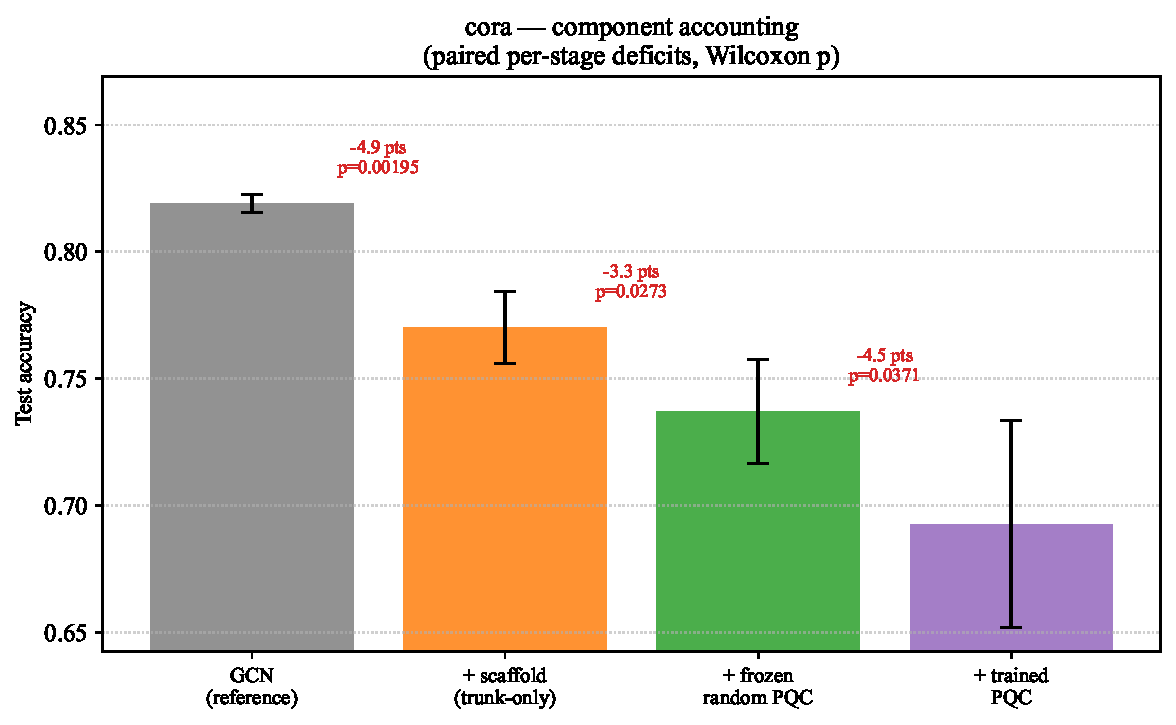
\includegraphics[width=0.75\textwidth]{figs/cora_waterfall.pdf}
\caption{Component-accounting waterfall on Cora (confirmatory). Each bar is a configuration swap from the previous one; annotations give the paired step size and Wilcoxon $p$. The decomposition sums exactly to the GCN$\to$NEMA-Q deficit.}
\label{fig:waterfall}
\end{figure}

Three observations. The scaffold itself costs 4.9 points, and the decomposition splits it: 3.1 points is the price of hyperbolic geometry (GCN vs.\ the dedicated HGCN baseline) and the remaining 1.8 points is scaffold overhead proper --- trunk-only lands significantly below even HGCN ($p=0.039$). Attaching a random frozen circuit costs a further 3.3 points. \emph{Training} that circuit costs 4.5 more --- the single largest attributable step below the reference is the one that standard practice assumes is beneficial. (The pilot population, seeds 0--9, gave the same decomposition within a point at every stage.)

\begin{figure}[t]
\centering
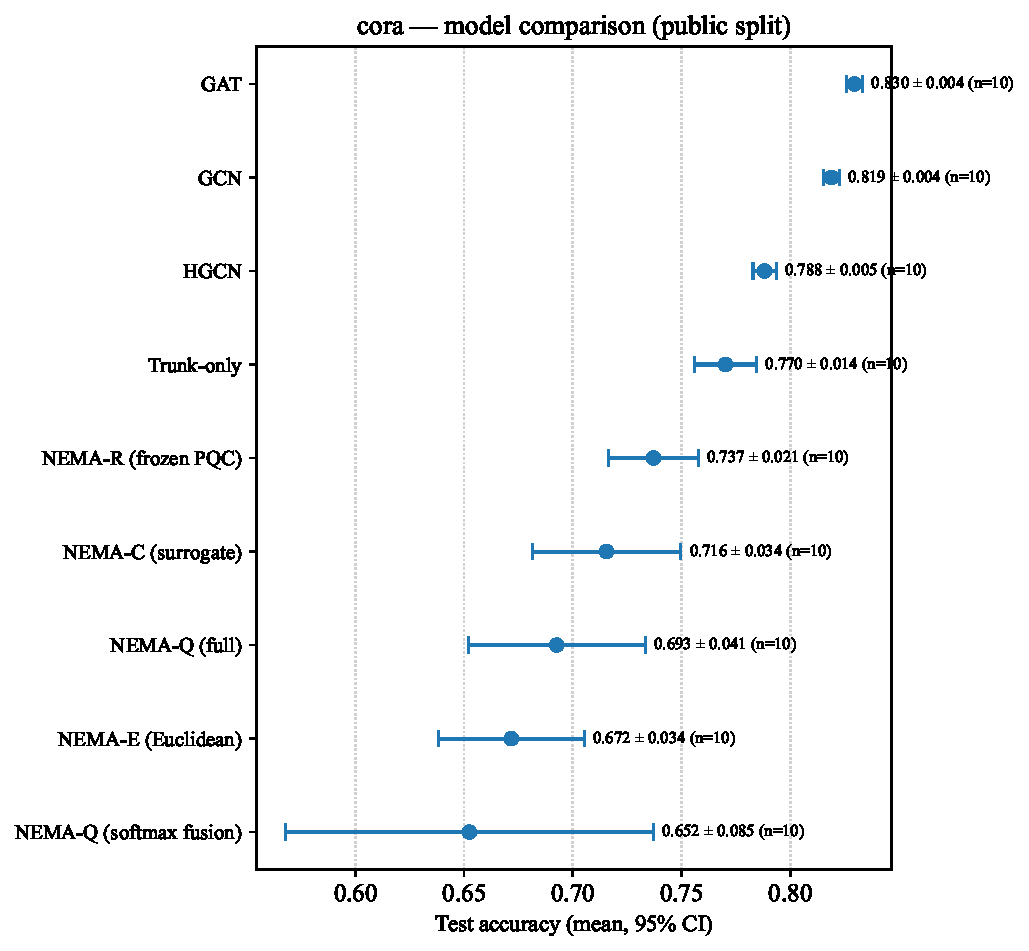
\includegraphics[width=0.49\textwidth]{figs/cora_forest.pdf}\hfill
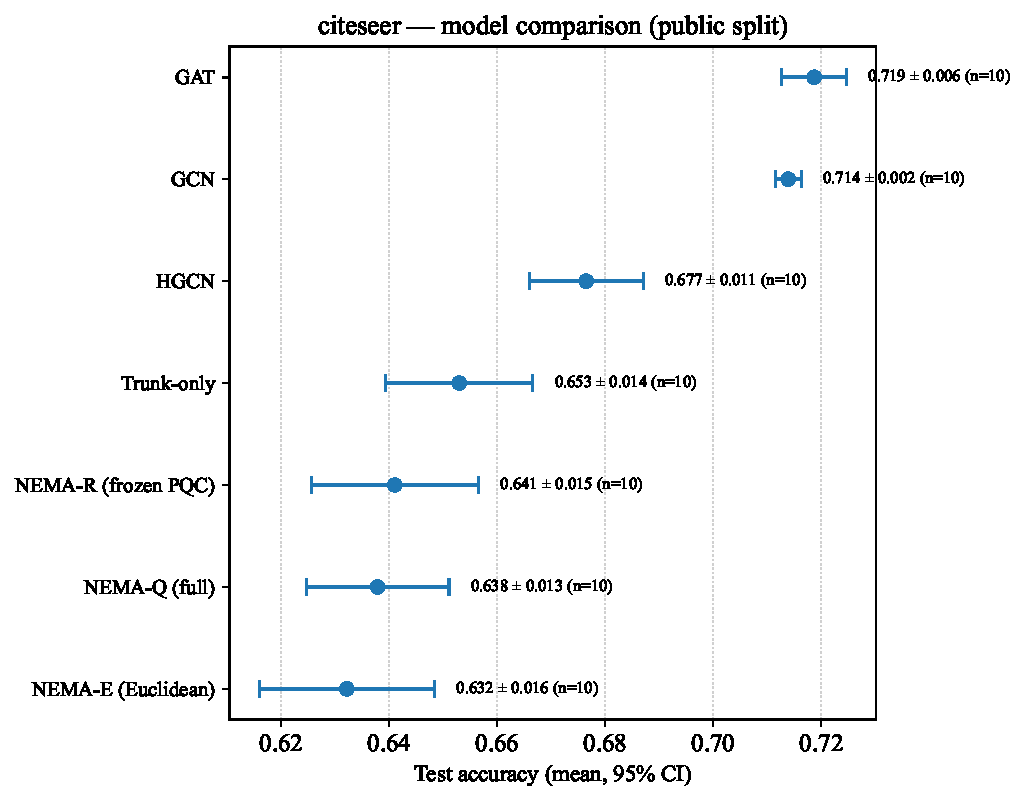
\includegraphics[width=0.49\textwidth]{figs/citeseer_forest.pdf}\\[2pt]
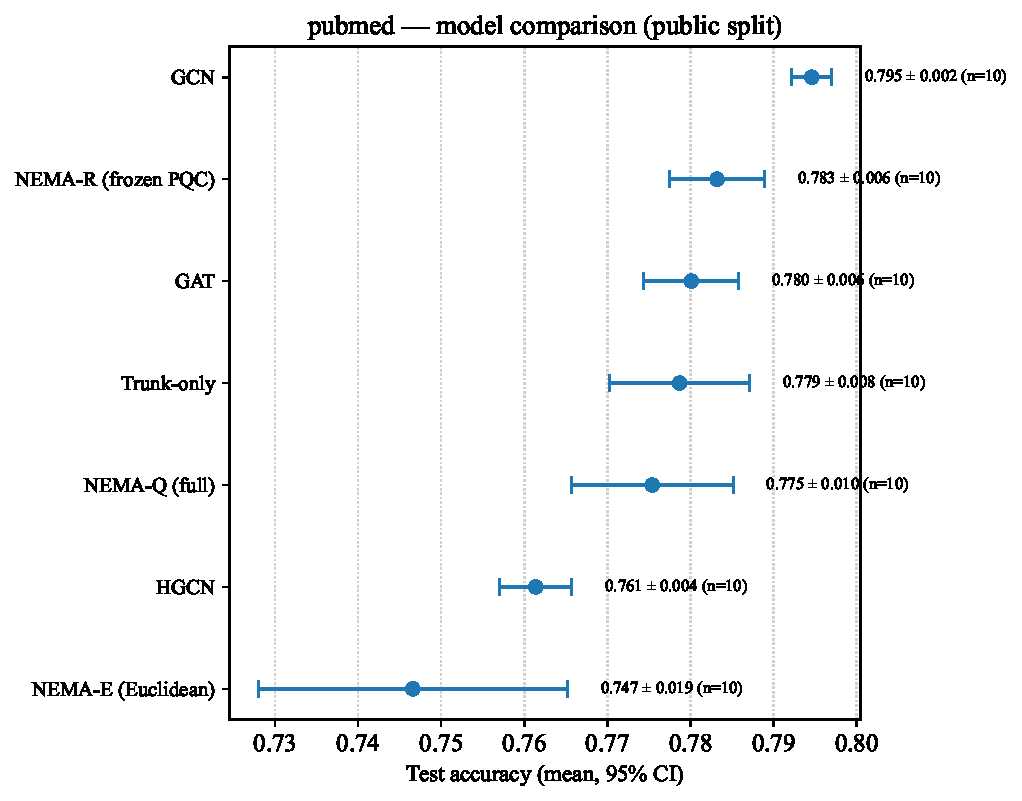
\includegraphics[width=0.49\textwidth]{figs/pubmed_forest.pdf}\hfill
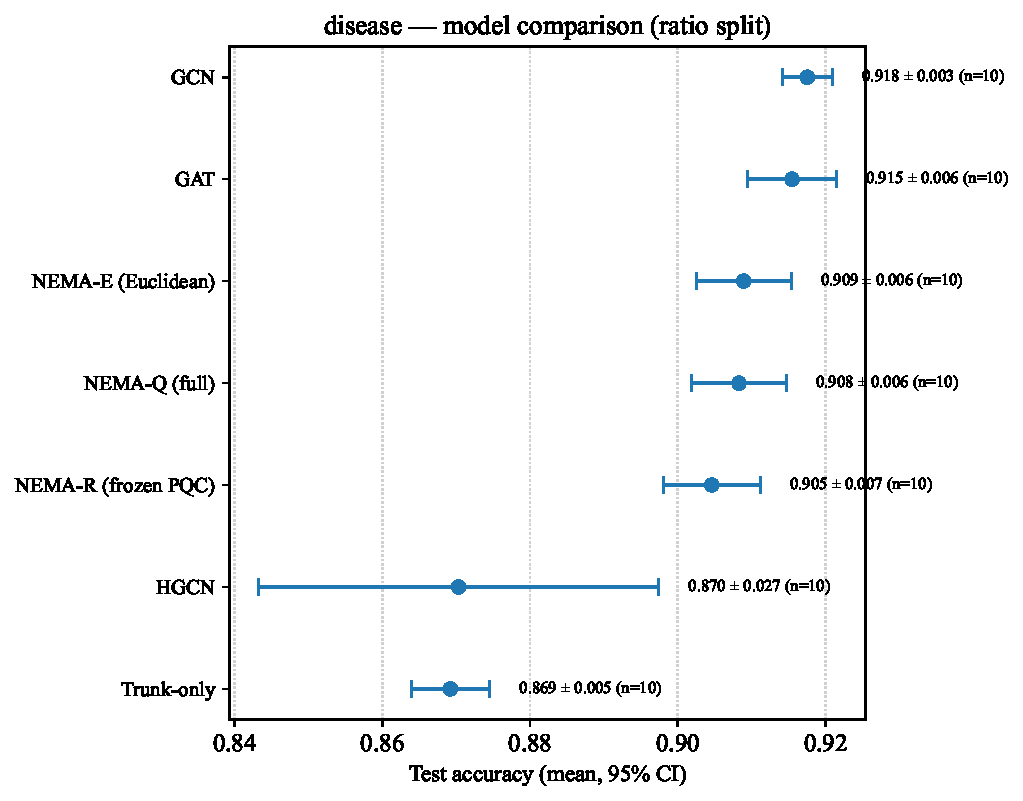
\includegraphics[width=0.49\textwidth]{figs/disease_forest.pdf}
\caption{Forest plots, one panel per dataset: test accuracy (mean $\pm$ 95\% CI over 10 paired confirmatory seeds) for all baselines, NEMA-Q, and every configuration-swap control under that dataset's locked recipe.}
\label{fig:forest}
\end{figure}

\subsection{H5: frozen matches or beats trained}\label{sec:h5}

Confirmatory (seeds 10--19), one-sided Wilcoxon (frozen $\ge$ trained), Holm--Bonferroni within the H5 family (Table~\ref{tab:h5}, Fig.~\ref{fig:h5paired}).

\begin{table}[t]
\centering
\caption{H5 --- frozen-random vs.\ trained PQC under an identical scaffold (confirmatory). One-sided Wilcoxon (frozen $\ge$ trained); Holm--Bonferroni within the four-dataset family.}
\label{tab:h5}
\footnotesize
\begin{tabular}{@{}lccccccc@{}}
\toprule
Dataset & Trained & Frozen & Diff & Wins & $p$ (raw) & $p$ (Holm) & $d$ \\
\midrule
Cora & $0.693\pm0.057$ & $0.737\pm0.029$ & $+4.5$ & 8/10 & 0.019 & 0.074 & $0.87$ \\
Pubmed & $0.775\pm0.014$ & $0.783\pm0.008$ & $+0.8$ & 7/10 & 0.169 & 0.507 & $0.46$ \\
Citeseer (tuned) & $0.638\pm0.019$ & $0.641\pm0.022$ & $+0.3$ & 4/10 & 0.577 & 1.0 & $0.11$ \\
Disease (tuned) & $0.908\pm0.009$ & $0.905\pm0.009$ & $-0.4$ & 4/10 & 0.837 & 1.0 & $-0.31$ \\
\bottomrule
\end{tabular}
\end{table}

The registered falsifier --- trained significantly better on a majority of datasets --- is approached nowhere: the trained circuit does not significantly beat its frozen control on a single dataset, while the frozen control is ahead in mean on three of four and significantly ahead on Cora at the uncorrected level (family-corrected $p=0.074$, marginal). The pilot population showed the same ordering with larger gaps (Cora $+3.9$, 10/10 seeds; Citeseer $+1.4$, $p=0.027$), so across twenty independent seeds per dataset the qualitative statement is stable: freezing is never worse, and on the dataset where the hybrid struggles most it is reliably better. Section~\ref{sec:discussion} discusses mechanism; Sect.~\ref{sec:failure} supplies the input-regime half of it.

\begin{figure}[t]
\centering
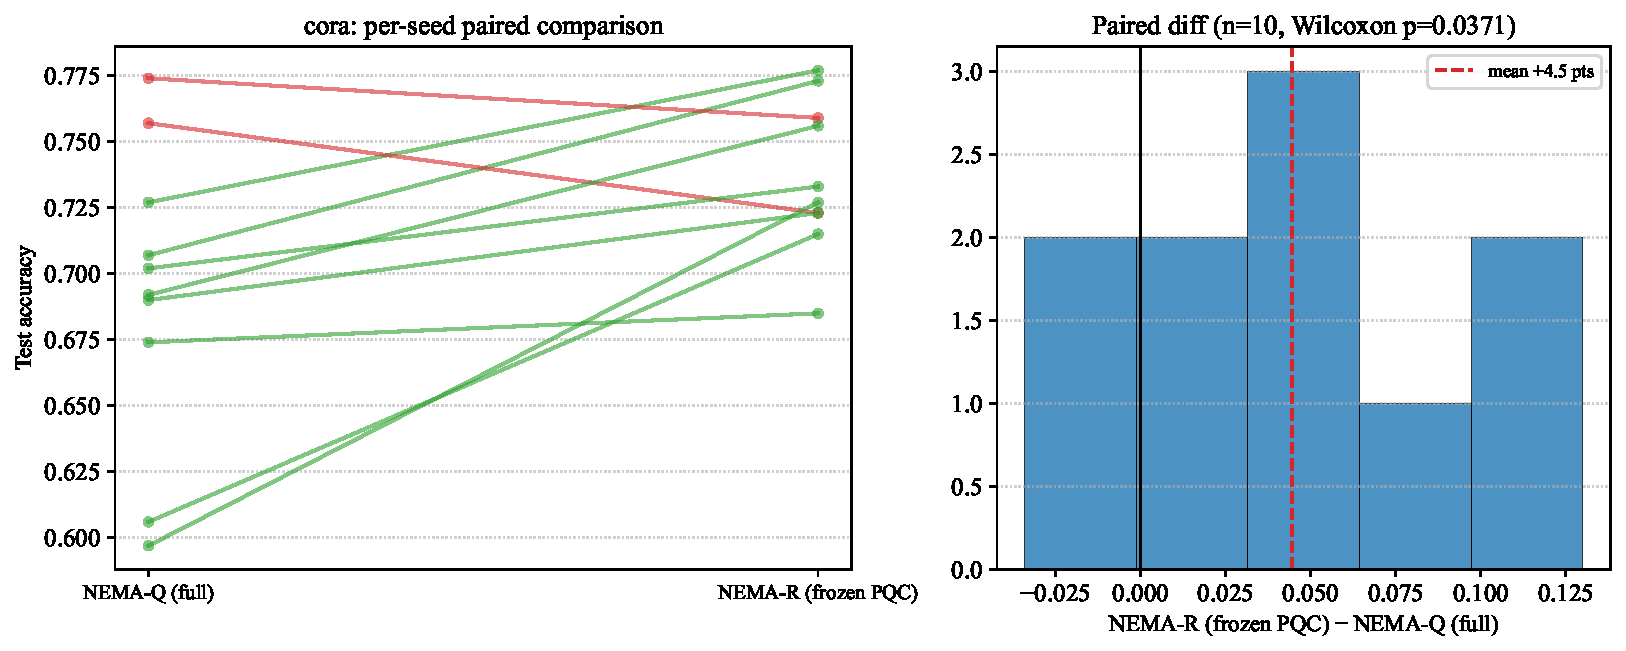
\includegraphics[width=0.49\textwidth]{figs/cora_paired_frozen_vs_trained.pdf}\hfill
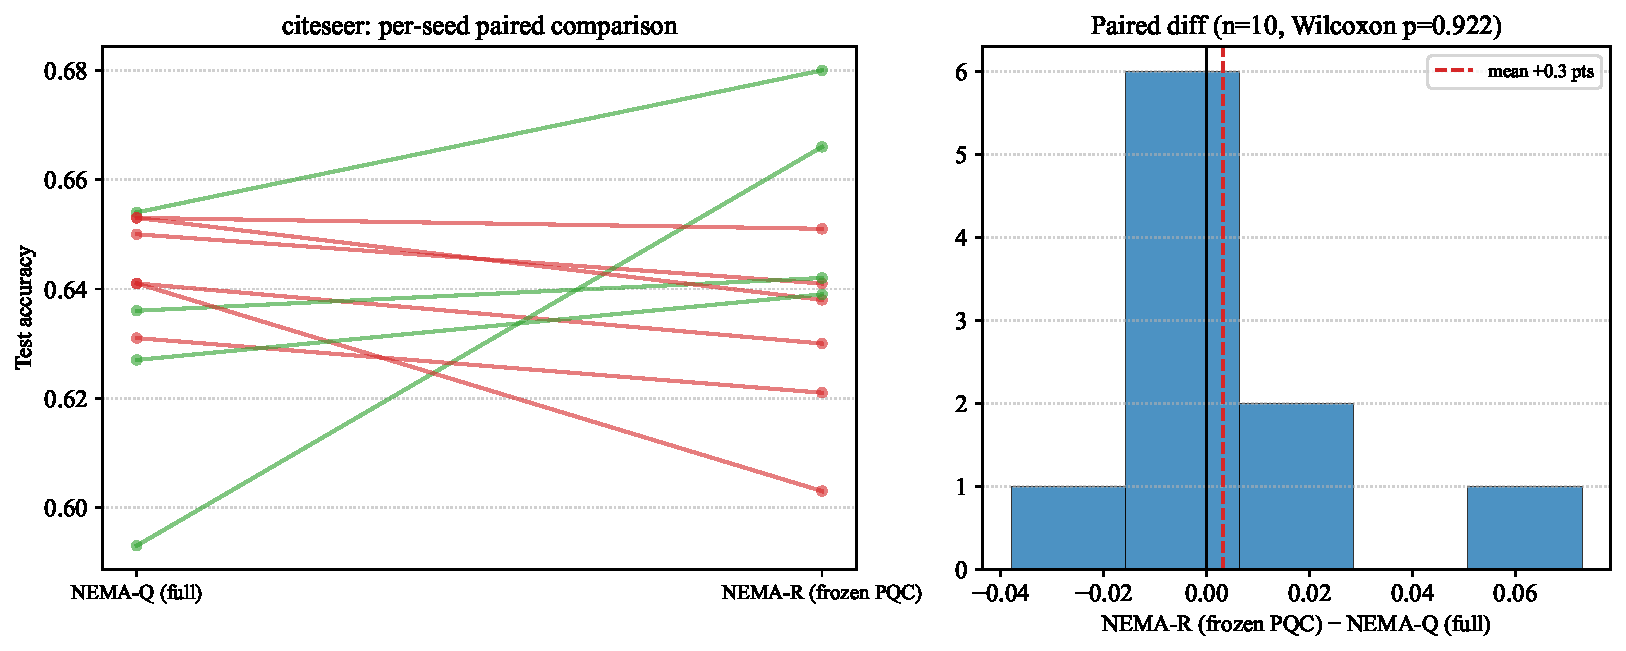
\includegraphics[width=0.49\textwidth]{figs/citeseer_paired_frozen_vs_trained.pdf}\\[2pt]
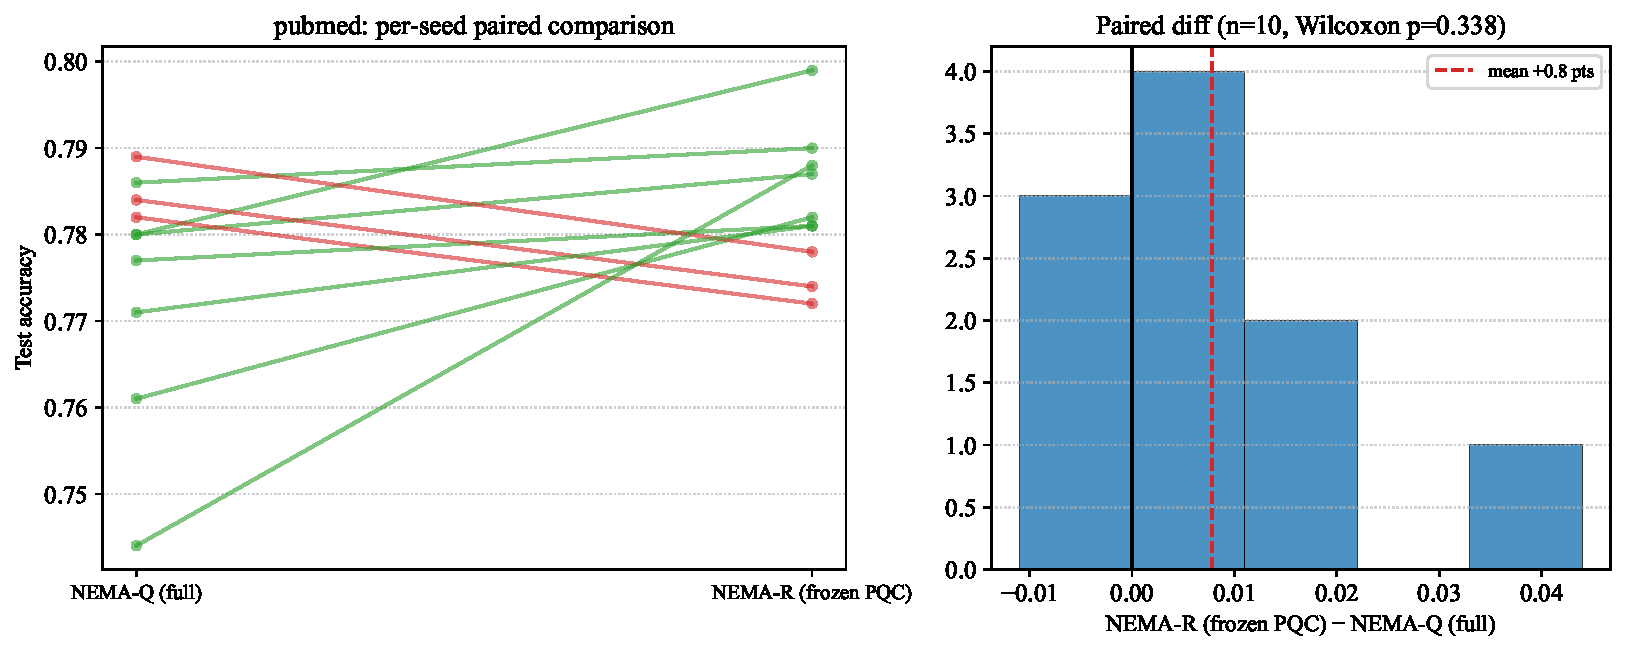
\includegraphics[width=0.49\textwidth]{figs/pubmed_paired_frozen_vs_trained.pdf}\hfill
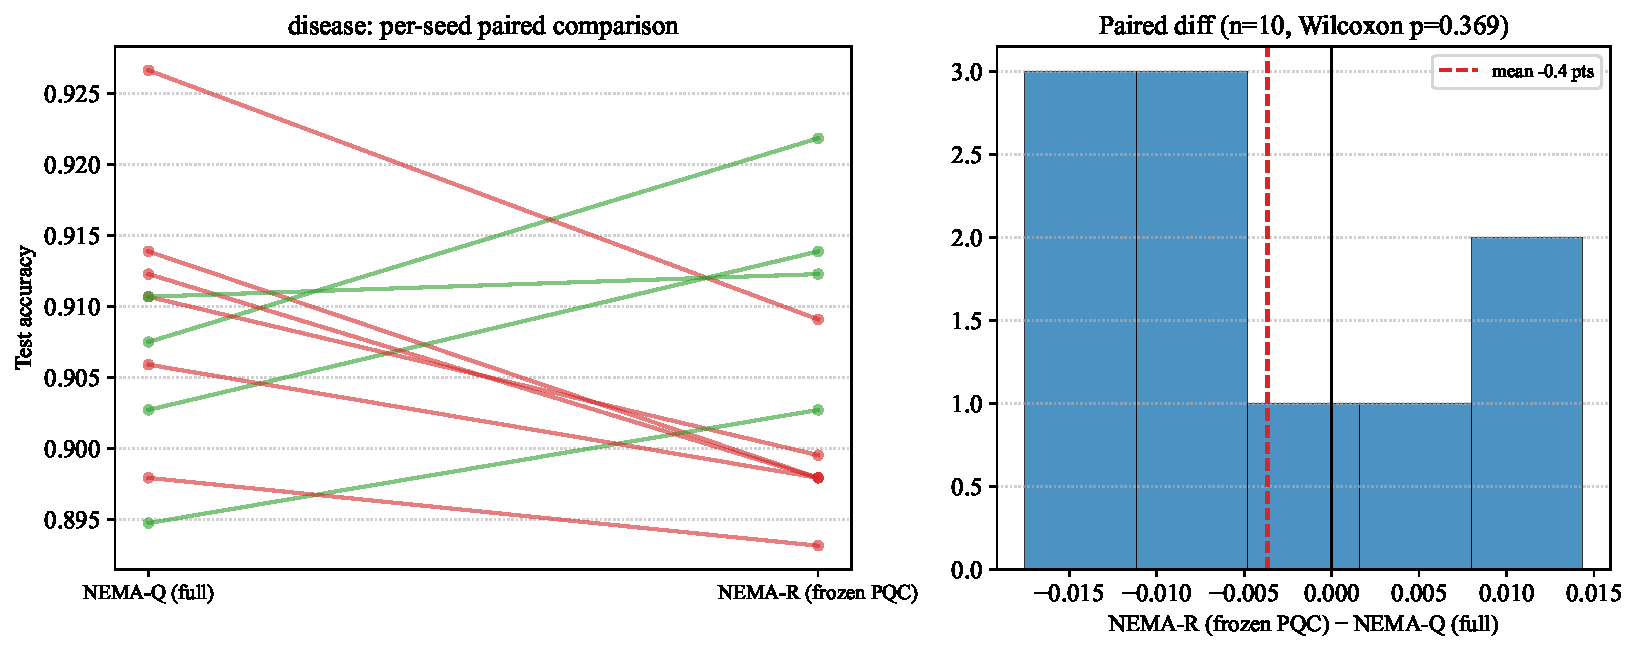
\includegraphics[width=0.49\textwidth]{figs/disease_paired_frozen_vs_trained.pdf}
\caption{H5 paired-seed plots, one panel per dataset: per-seed test accuracy of trained PQC (NEMA-Q) vs.\ frozen-random PQC (NEMA-R) connected by seed. Slope direction, not vertical position, carries the H5 verdict.}
\label{fig:h5paired}
\end{figure}

\subsection{Remaining preregistered hypotheses}\label{sec:remaining}

\paragraph{H2 (quantum vs.\ surrogate): falsified} At standard label rates on Cora, the parameter-matched classical surrogate reaches $0.716\pm0.048$ (confirmatory) --- statistically indistinguishable from the trained PQC (paired $p=0.61$) and, if anything, ahead in mean ($+2.3$ points, n.s.). The pilot population's variance asymmetry (surrogate $2.7\times$ less stable, Levene $p=0.02$) did not replicate (confirmatory sd ratio $0.84$, Levene $p=0.76$), so we do not report a stability difference. The registered low-label half (5 labels per class, cora/citeseer/pubmed, seeds 10--19, seeded shared splits; declared in a dated pre-run amendment) is also null: the PQC's mean advantage is positive on all three datasets ($+2.6$, $+0.7$, $+0.1$ points; PQC $0.570\pm0.039$ vs.\ surrogate $0.544\pm0.063$ on Cora) but significant on none (one-sided $p=0.16$ / $0.46$ / $0.75$; pooled Stouffer $p=0.41$). The registered falsifier --- surrogate matches the PQC at all label rates --- is triggered. The dequantization reading stands at every label rate tested: nothing the trained circuit does on these tasks exceeds a matched classical branch.

\paragraph{The completed primary family} With H2 run, the registered family reads: H5 (best dataset, Cora) raw $p=0.019 \to$ Holm $0.056$; H1-pooled $0.040 \to 0.080$; H2 $0.408$. No member survives family-wise correction at $\alpha=0.05$. Component accounting reports this as the result: on this suite, every registered positive claim about the exotic components is marginal or null once the full testing plan is accounted for.

\paragraph{H3 (trainability telemetry)} The relative criterion --- PQC circuit-weight gradient variance within two orders of magnitude of the healthiest classical branch on $\ge 9/10$ seeds --- passes on the three citation networks (10/10 each, confirmatory) but \textbf{fails on Disease (6/10)}: on the dataset where the quantum branch's attribution is input-dominated (Sect.~\ref{sec:qoa}), its gradients also intermittently collapse relative to the classical reference. The Citeseer result remains the instructive one: H3 passes on the collapsed pilot runs, certifying that gradients \emph{flow} while Sect.~\ref{sec:failure} shows flowing gradients can carry no per-node information. Trainability telemetry is necessary but not sufficient --- and on Disease not even reliably attained.

\paragraph{H4 (gate--attribution validity): falsified} Pooled over datasets and seeds ($n=40$ confirmatory NEMA-Q runs), the Spearman correlation between fusion-gate mass and leave-branch-out deltas is $\rho=0.47$ for the geo branch and $\rho=0.37$ for the quantum branch --- both at or below the registered $0.5$ threshold, with large per-seed spread (individual runs range from $-0.99$ to $+0.99$). Per-dataset means: geo $0.62/0.27/0.51/0.49$ and q $0.47/0.37/0.50/0.11$ on Cora/Citeseer/Pubmed/Disease. The registered falsifier ($\rho \le 0.5$) is triggered: gate mass is not a trustworthy readout of branch usefulness. This confirms quantitatively what Sect.~\ref{sec:failure}'s uniform-gate-over-a-dead-branch already showed qualitatively --- gates track branch \emph{usage}, not branch \emph{usefulness} --- and it is why QOA attributes against measured observables rather than against gates.

\subsection{Fusion stability}\label{sec:fusion}

Softmax fusion is a variance pathology, not (reliably) a mean one. Confirmatory: $0.652\pm0.118$ on Cora versus $0.693\pm0.057$ residual --- the mean gap ($+4.0$ points toward residual) is not significant ($p=0.70$), but the seed-level spread doubles (sd ratio $2.1$, Levene $p=0.023$), with softmax seeds ranging $0.44$--$0.77$. The pilot population showed the same variance signature more extremely (sd ratio ${\sim}5$, Levene $p=0.008$, and a 10.4-point mean gap that did not replicate in magnitude). We therefore claim only what both populations support: softmax competition makes training outcome a lottery over seeds, and residual gating with a closed-gate initialization removes that lottery. The pilot's classical surrogate exhibited the same instability under softmax, so this is a fusion pathology, not a quantum one. All headline configurations use residual fusion.

\begin{figure}[t]
\centering
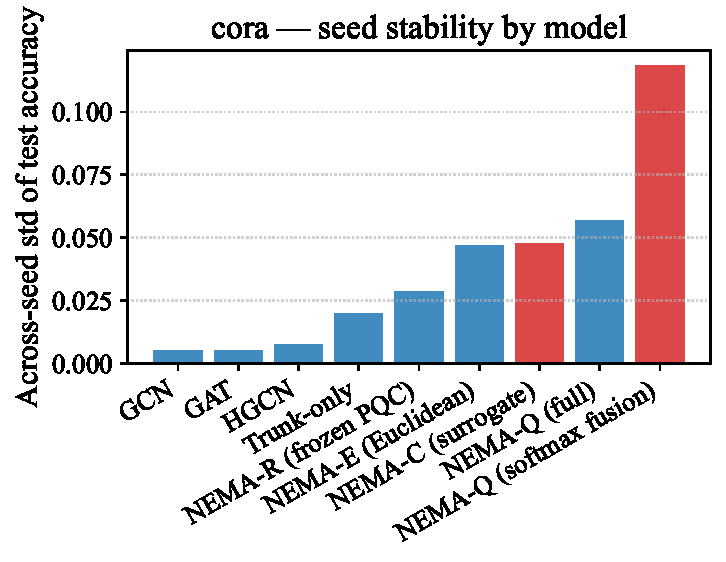
\includegraphics[width=0.49\textwidth]{figs/cora_stability.pdf}\hfill
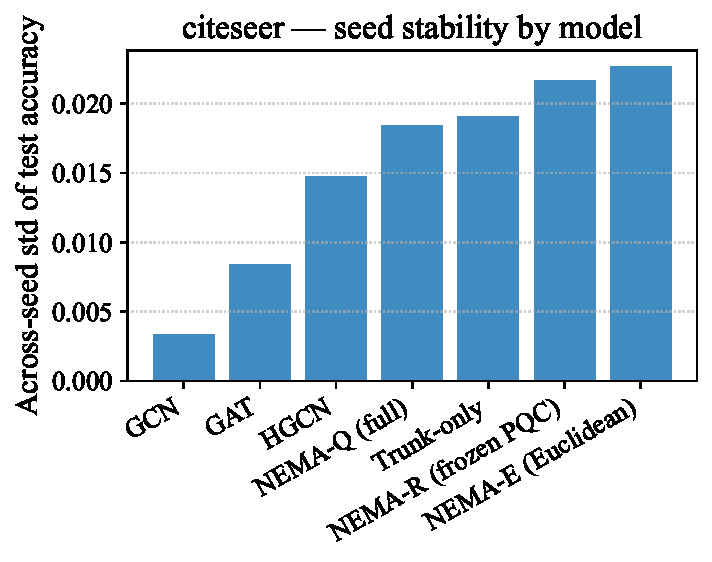
\includegraphics[width=0.49\textwidth]{figs/citeseer_stability.pdf}\\[2pt]
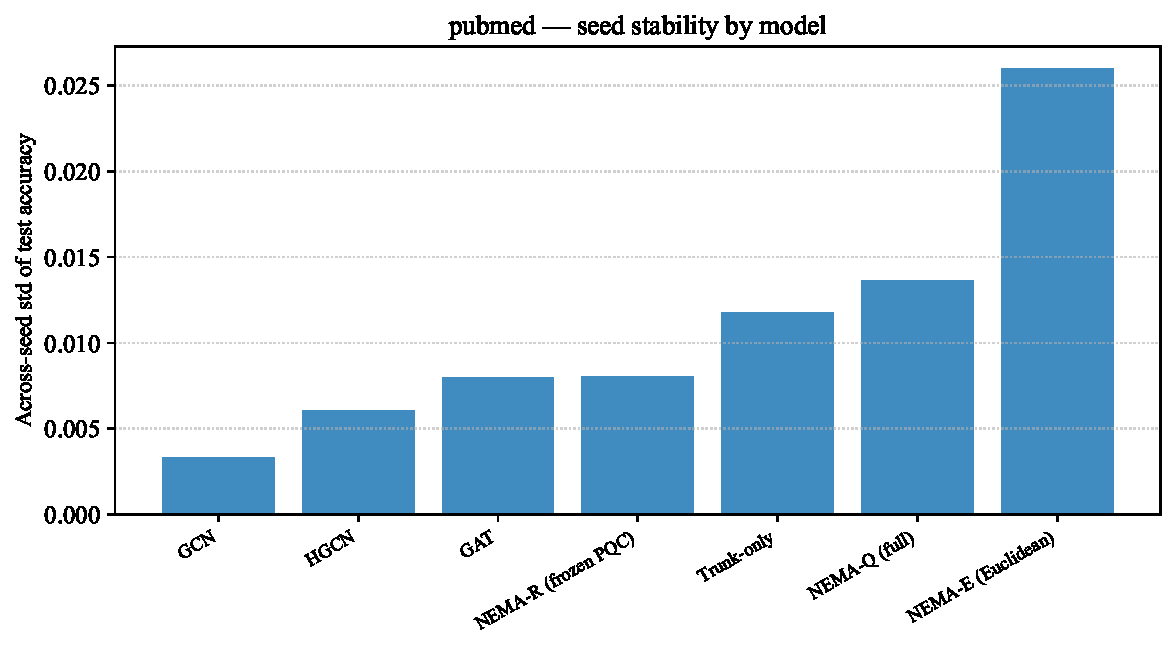
\includegraphics[width=0.49\textwidth]{figs/pubmed_stability.pdf}\hfill
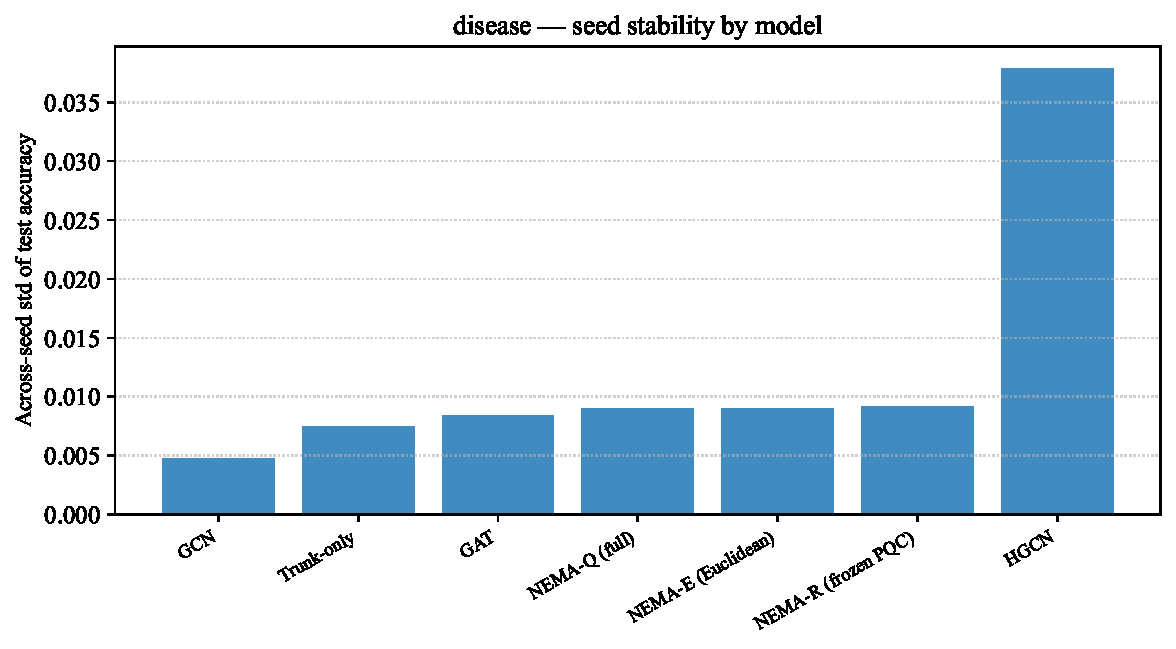
\includegraphics[width=0.49\textwidth]{figs/disease_stability.pdf}
\caption{Seed-level stability, one panel per dataset: per-seed test accuracy distributions for residual vs.\ softmax fusion and for each control. Variance, not mean, separates the fusion modes.}
\label{fig:stability}
\end{figure}

\section{Results II: geometry --- the encoder works, the textbook mechanism does not}\label{sec:geometry}

Per-dataset paired gains (hyperbolic $-$ Euclidean, identical locked recipes; confirmatory, one-sided Wilcoxon as registered) are given in Table~\ref{tab:geometry} and Fig.~\ref{fig:geometry}.

\begin{table}[t]
\centering
\caption{H1 --- paired hyperbolic $-$ Euclidean gains under identical locked recipes (confirmatory).}
\label{tab:geometry}
\begin{tabular}{@{}lcccc@{}}
\toprule
Dataset & $\delta$ & Gain & $p$ (one-sided) & $d$ \\
\midrule
Disease  & 0.000 & $-0.1$ & 0.455 & $-0.05$ \\
Cora     & 0.356 & $+2.1$ & 0.302 & $0.23$ \\
Pubmed   & 0.399 & $+2.9$ & 0.014 & $0.99$ \\
Citeseer & 0.550 & $+0.6$ & 0.254 & $0.22$ \\
\bottomrule
\end{tabular}
\end{table}

\begin{figure}[t]
\centering
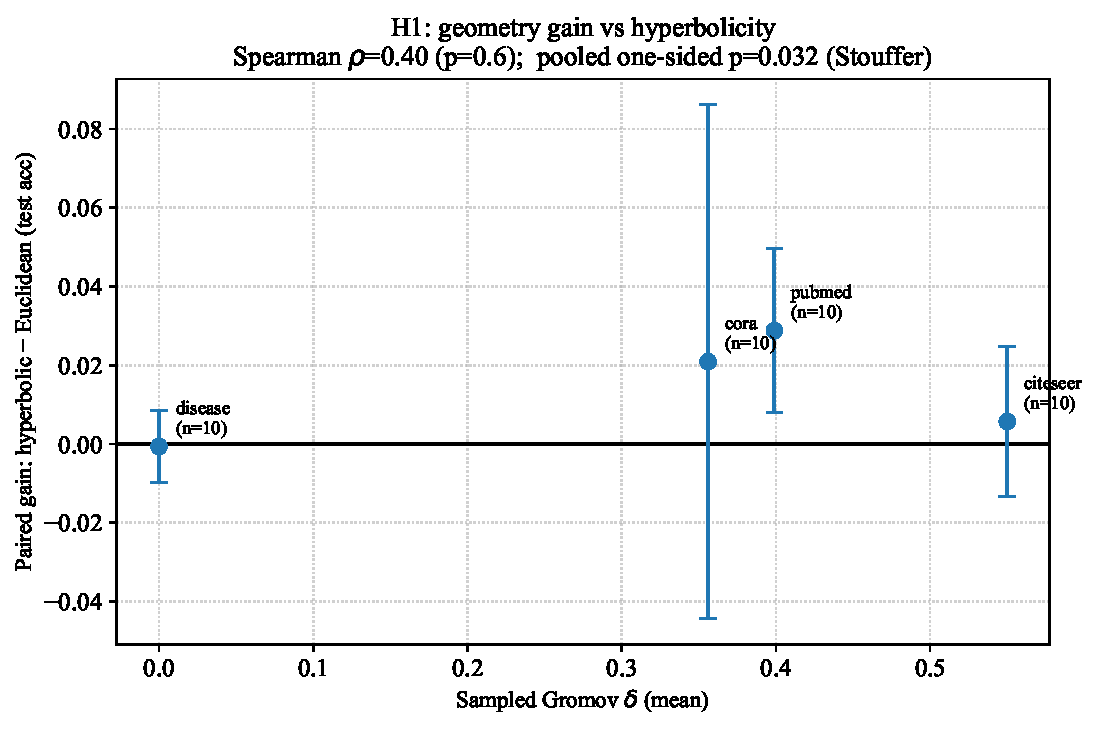
\includegraphics[width=0.6\textwidth]{figs/h1_geometry_delta.pdf}\\[2pt]
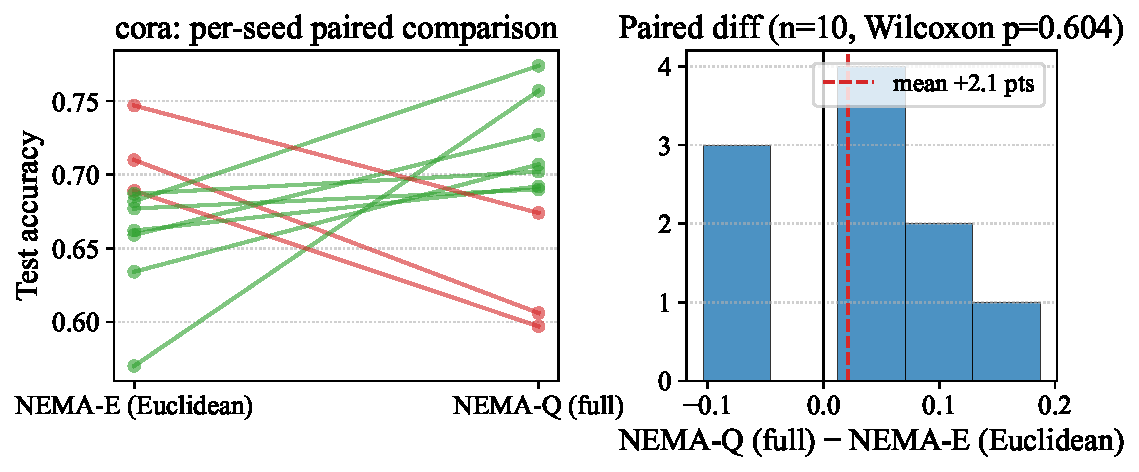
\includegraphics[width=0.49\textwidth]{figs/cora_paired_geometry.pdf}\hfill
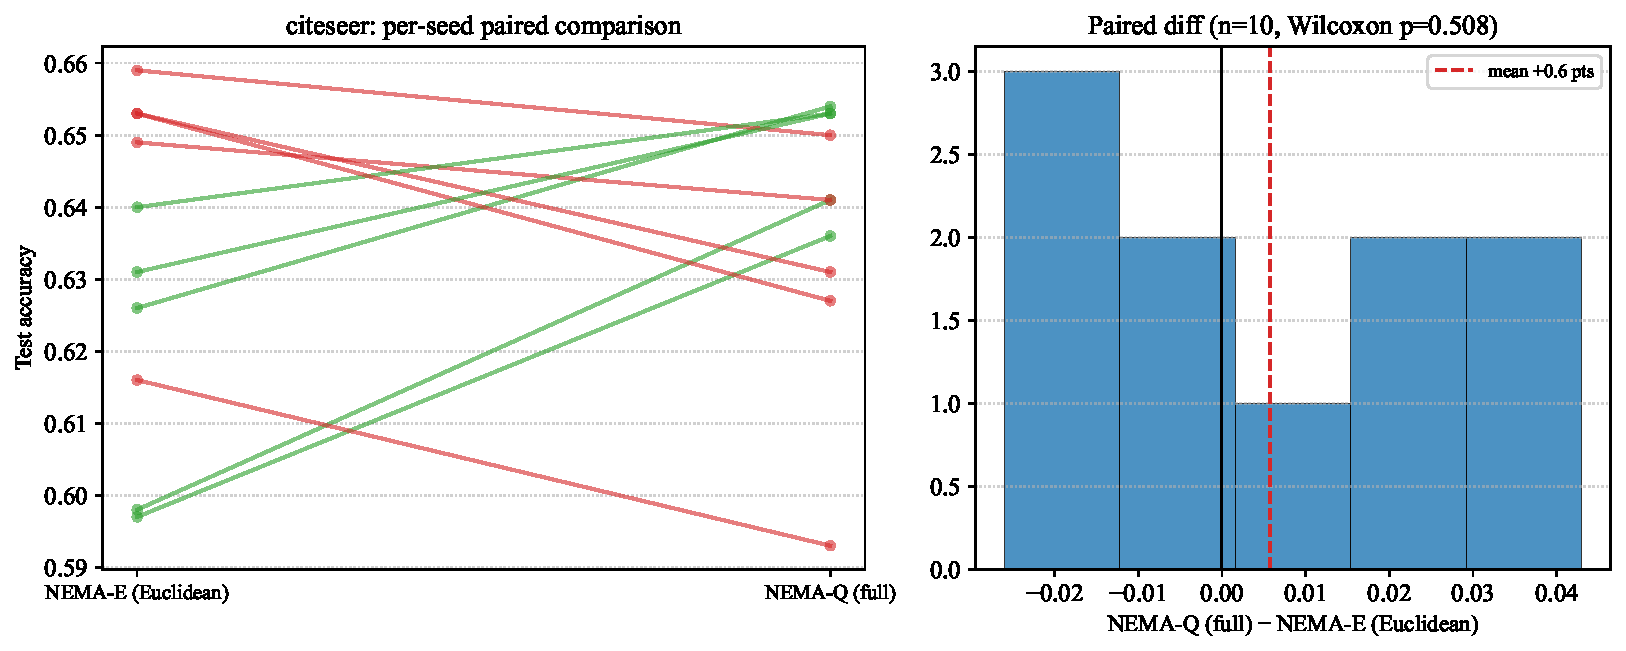
\includegraphics[width=0.49\textwidth]{figs/citeseer_paired_geometry.pdf}\\[2pt]
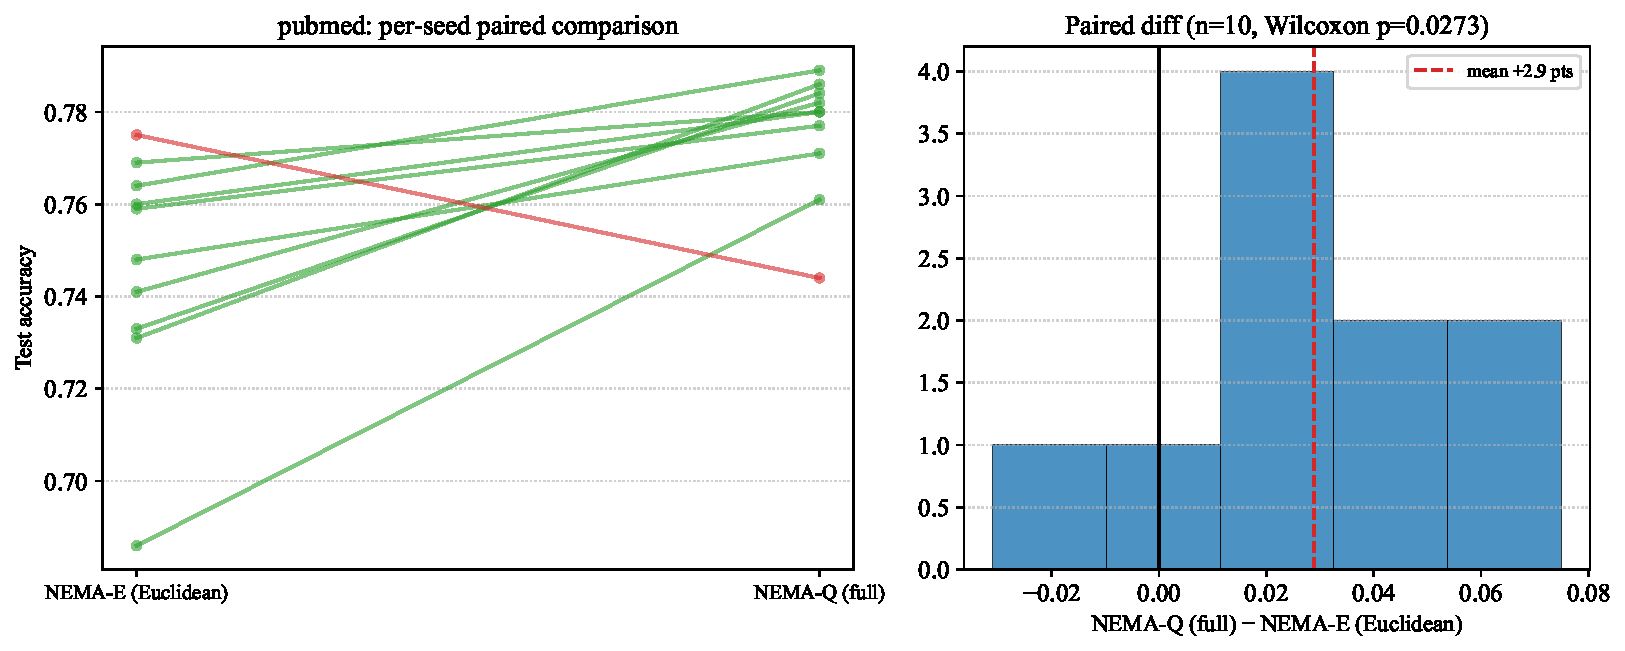
\includegraphics[width=0.49\textwidth]{figs/pubmed_paired_geometry.pdf}\hfill
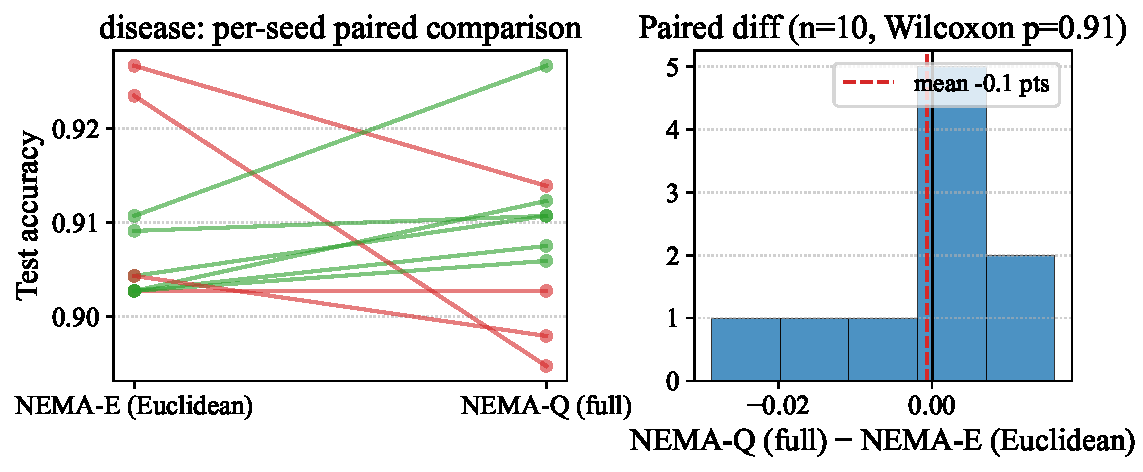
\includegraphics[width=0.49\textwidth]{figs/disease_paired_geometry.pdf}
\caption{Geometry $\times$ $\delta$. Top: paired hyperbolic$-$Euclidean gain (mean $\pm$ 95\% CI) against dataset $\delta_{\text{mean}}$; the preregistered H1(b) prediction is a negative slope, the observed trend is positive. The in-panel pooled annotation is the registered statistic (Stouffer over one-sided Wilcoxon tests). Bottom: per-dataset paired-seed plots (NEMA-Q vs.\ NEMA-E).}
\label{fig:geometry}
\end{figure}

\paragraph{H1(a) direction: holds on its registered falsifier, marginal under family correction} Stouffer-pooled one-sided $p=0.040$ ($Z=1.75$) across the four datasets under their locked recipes --- the registered falsifier (raw pooled $p \ge 0.05$) is not triggered, and the pooled direction is positive. Under the completed primary-family Holm correction, however, the pooled $p$ rises to $0.080$ (Sect.~\ref{sec:remaining}), so we do not claim family-wise significance. The pooled evidence is also weaker than the pilot suggested (pilot $p\approx0.004$, which mixed recipe conditions across datasets; the confirmatory number supersedes it). Only Pubmed reaches per-dataset significance ($p=0.014$, $d=0.99$).

\paragraph{H1(b) mechanism: falsified} The registered falsifier --- no negative $\delta$--gain correlation --- is triggered: the gains \emph{rise} with $\delta$ (confirmatory Spearman $\rho=+0.40$; the trend itself is not significant over four datasets, $p=0.60$, and we do not claim it is --- the informative datum is the zero gain on the exact tree). The outcome is robust across seed populations: the pilot showed the same positive trend with its largest gain on Citeseer ($\delta=0.550$), the confirmatory population with its only significant gain on Pubmed ($\delta=0.399$) --- in neither population does the gain concentrate at low $\delta$. On the exact tree --- where the mechanism story predicts its maximum --- the confirmatory gain is zero ($-0.1$, $p=0.455$) and a plain GCN outperforms the dedicated HGCN baseline by 4.7 points ($0.918\pm0.005$ vs.\ $0.870\pm0.038$, the HGCN additionally showing one majority-class-collapse seed). Whatever the hyperbolic encoder contributes on this suite, $\delta$-hyperbolicity does not predict it --- consistent with the geometry--task-alignment reading of hyperbolic gains \cite{alignment2026hyperbolic}. Learned curvature points the same way: the encoder relaxes toward flat or moderate curvature on the citation networks ($c\approx0.96$--$1.18$) and steepens only on Disease ($c\approx1.35$) where it earns no accuracy gain. We report this as a preregistered two-part outcome: direction confirmed, mechanism rejected --- a combination a single-dataset study could not produce.

\section{Results III: a failure mode of gated fusion, diagnosed and repaired}\label{sec:failure}

Under the default recipe, NEMA-Q collapses on Citeseer: $0.508\pm0.063$ versus $0.717$ for GCN, with early stopping firing within ${\sim}40$ effective epochs, whole classes dropped (minimum per-class F1 reaching $0.0$), and validation tracking test --- a training failure, not overfitting (pilot).

\paragraph{Mechanism} Per-branch gradient telemetry from the failed runs shows a three-order-of-magnitude imbalance: hyperbolic-branch gradient variance ${\sim}10^{-11}$ (starved), trunk ${\sim}10^{-8}$, quantum branch $10^{-7}$--$10^{-6}$ (loudest in the network). The quantum branch's input is the culprit: Citeseer's sparse features (density $0.008$, the suite's lowest) drive the compressed angle embedding to the lowest per-dimension variance of any dataset ($\sigma=0.005$ vs.\ $0.013$--$0.016$), so the circuit outputs are nearly constant across nodes (output $\sigma=0.013$) while the branch's parameters still receive large gradients. The fusion gate admits this channel \emph{uniformly} --- gate value $0.177\pm0.005$ across all nodes --- a pathway carrying no per-node information but maximal gradient noise into the shared head. Notably, the entire angle range used is $\pm0.15$ of the available $\pm\pi$ on every dataset: the embedding operates in a narrow near-linear regime everywhere, and Citeseer merely falls below the usable-variance floor. This observation independently rationalizes H5 (Sect.~\ref{sec:discussion}).

\paragraph{Alternative tested and rejected} Citeseer is also the most fragmented graph in the suite (largest component 64\% of nodes). Fragmentation, however, does not explain the failure: in the collapsed model, isolated test nodes are classified no worse than connected ones ($0.500$, $n=12$, vs.\ $0.401$, $n=988$) --- a small isolated-node sample, but the effect required for fragmentation to explain a 21-point collapse would point sharply the other way.

\paragraph{Repair} The mechanism predicts the fix: strengthen per-branch supervision so branches learn discriminative features regardless of gate dynamics. A validation-only sweep confirms monotone recovery in the auxiliary-loss weight (val $0.505 \to 0.661$ as aux $0.3 \to 2.0$, with quieter gate initialization $-4$ and lr $0.005$; pilot sweep). Under the locked recipe the confirmatory population reaches $0.638\pm0.019$ --- within 1.5 points of trunk-only ($0.653\pm0.019$), with no class collapse and normal convergence, versus $0.508\pm0.063$ collapsed. The repair recovers the trunk; it does not make the exotic branches help. The same recipe was applied to all Citeseer hybrid variants for the paired comparisons of Sects.~\ref{sec:accounting}--\ref{sec:geometry}.

\paragraph{Precondition (branch signal-variance preflight)} Stable gated fusion requires each branch to retain per-node signal variance at its output; for angle-embedded quantum branches this is measurable \emph{before training} from the compressed-input variance. We propose reporting this statistic as a standard preflight check for hybrid architectures.

\section{Quantum Observable Attribution, with its own audit}\label{sec:qoa}

QOA attributes each node's predicted-class logit to the measured observables at the quantum--classical boundary. Let $o_i \in \mathbb{R}^n$ be node $i$'s Pauli-Z expectation vector (Sect.~\ref{sec:arch}) and $\hat{y}_i$ its predicted class. QOA substitutes the observable tensor into the forward graph as a leaf variable and differentiates the predicted-class logit through projection, fusion, and head:
\begin{equation}
\mathrm{QOA}(i,k) \;=\; \frac{\partial\, \ell_{i,\hat{y}_i}}{\partial\, o_{ik}}\; \cdot\; o_{ik},
\end{equation}
gradient $\times$ input over the observable vector. Two properties matter. First, the attribution target is neither the circuit's gates \cite{heese2025shapley} nor the input features, but the interface where quantum information becomes classical feature --- so QOA answers the hybrid-specific question: \emph{which physical measurements does the classical readout actually use?} Second, because $o_i$ is recomputed exactly (statevector simulation) and substituted as a leaf, the method needs no relaxation or sampling; it is exact for the model as trained.

The conference version's reviewers noted, correctly, that gradient saliency without faithfulness evidence is decoration. The extension supplies a three-check harness, run per dataset on the trained models:
\begin{enumerate}
\item \textbf{Masking faithfulness:} zeroing the top-attributed observable per node ($k=1$) must reduce the predicted-class logit more than zeroing the bottom-attributed one: pass iff mean drop(top) $>$ mean drop(bottom) over test nodes.
\item \textbf{Perturbation test:} Gaussian noise ($\sigma=0.25$) injected on the top-attributed observable must flip more predictions than on the bottom-attributed one: pass iff flip-rate(top) $>$ flip-rate(bottom).
\item \textbf{Model-randomization sanity check} \cite{adebayo2018sanity}: re-randomizing fusion and head must collapse the attribution pattern: pass iff Spearman $|\rho|$ between original and randomized attributions $< 0.5$. A method that survives randomization is reading input structure, not the model.
\end{enumerate}

Across the four datasets, QOA passes 11 of 12 checks in the pilot population: masking and perturbation faithfulness hold everywhere (top-attributed observables produce strictly larger logit drops and higher flip rates than bottom-attributed ones on every dataset; per-dataset magnitudes in Fig.~\ref{fig:faithfulness}), and randomization passes on Cora, Citeseer, and Pubmed. The randomization check was re-run per seed in the confirmatory population and replicates exactly: mean $|\rho| = 0.24 / 0.10 / 0.18$ on Cora / Citeseer / Pubmed (pass) versus $0.56$ on Disease (fail). The single failure is thus stable across twenty seeds: on a two-class task whose quantum branch operates in the near-constant regime of Sect.~\ref{sec:failure} --- and whose gradient telemetry intermittently fails H3 (Sect.~\ref{sec:remaining}) --- the attribution pattern is dominated by input structure rather than learned parameters, precisely the pathology the Adebayo check exists to expose. We therefore report QOA as validated on the three citation networks and flag Disease attributions as input-dominated rather than model-specific. A harness that can fail, and does --- consistently, on the same dataset, in both seed populations --- is the point: attribution methods should earn trust per dataset, not by construction.

\begin{figure}[t]
\centering
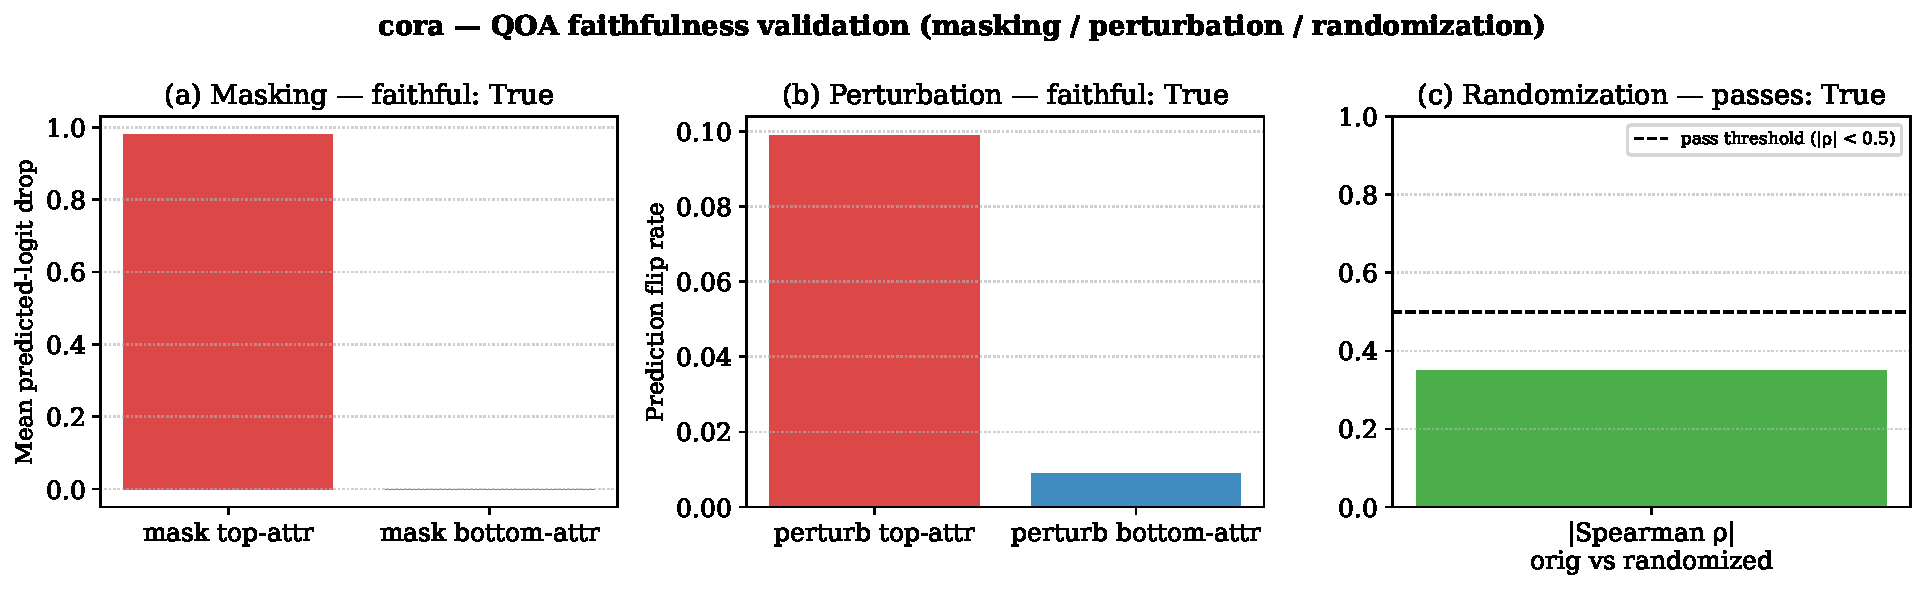
\includegraphics[width=0.49\textwidth]{figs/cora_xai_02_qoa_faithfulness.pdf}\hfill
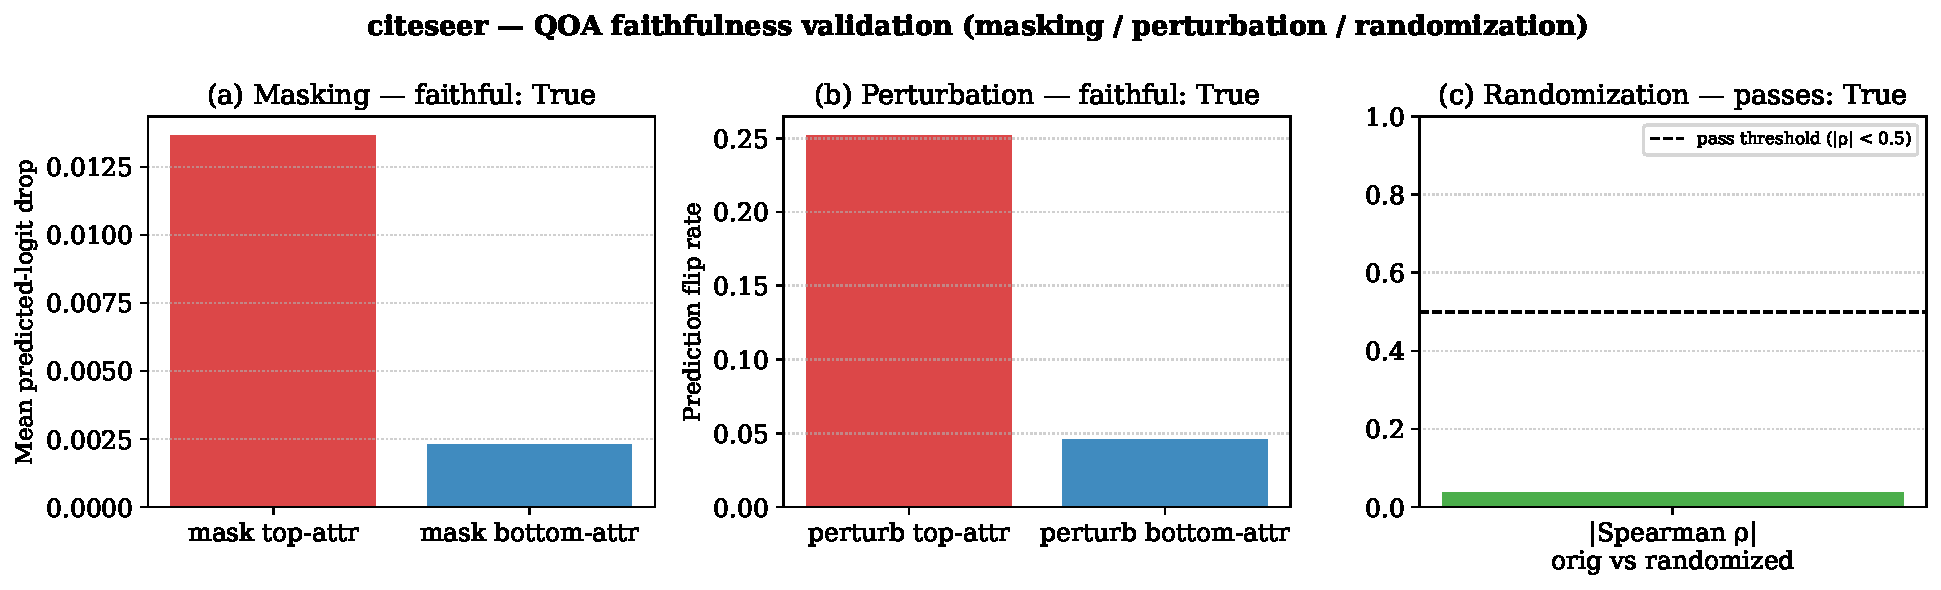
\includegraphics[width=0.49\textwidth]{figs/citeseer_xai_02_qoa_faithfulness.pdf}\\[2pt]
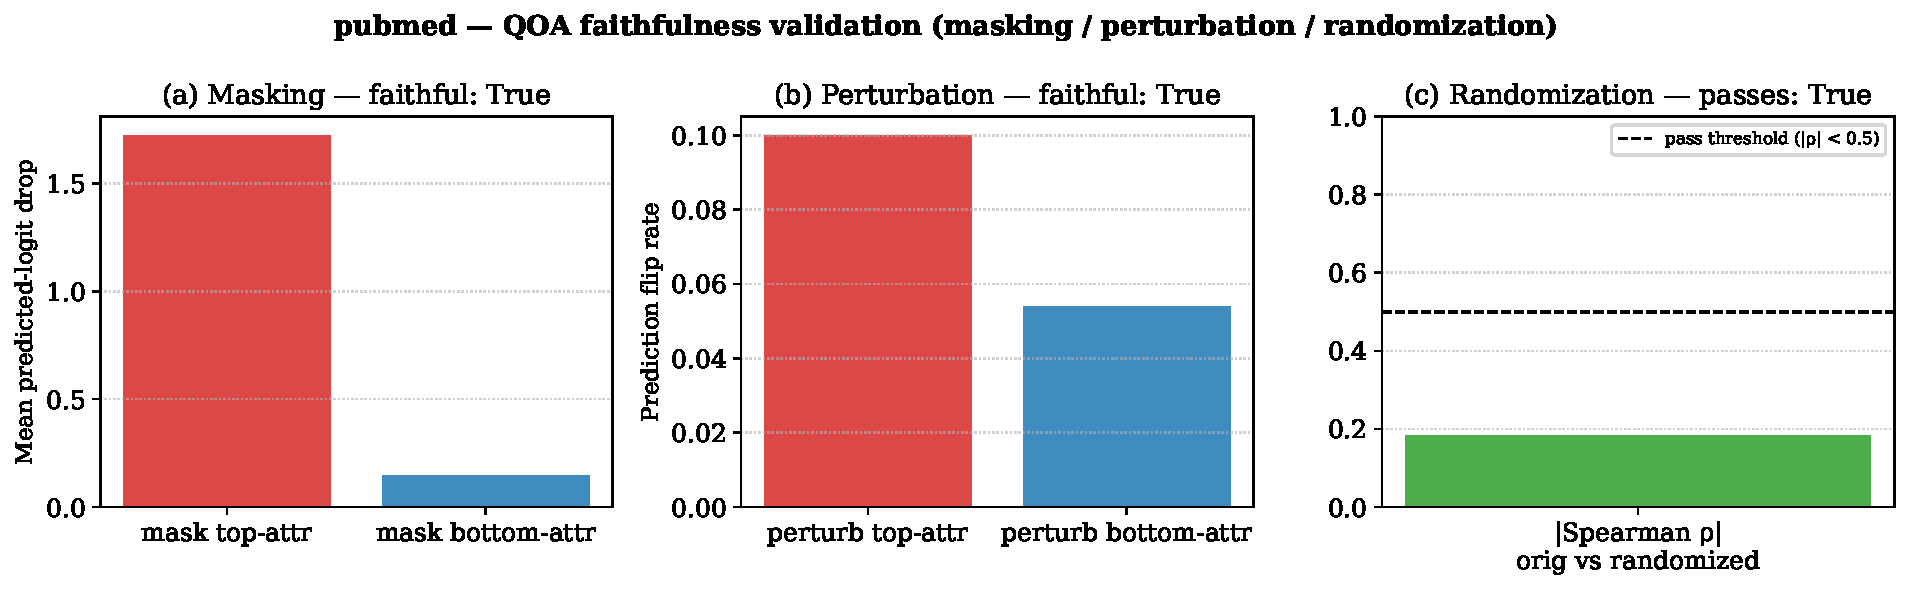
\includegraphics[width=0.49\textwidth]{figs/pubmed_xai_02_qoa_faithfulness.pdf}\hfill
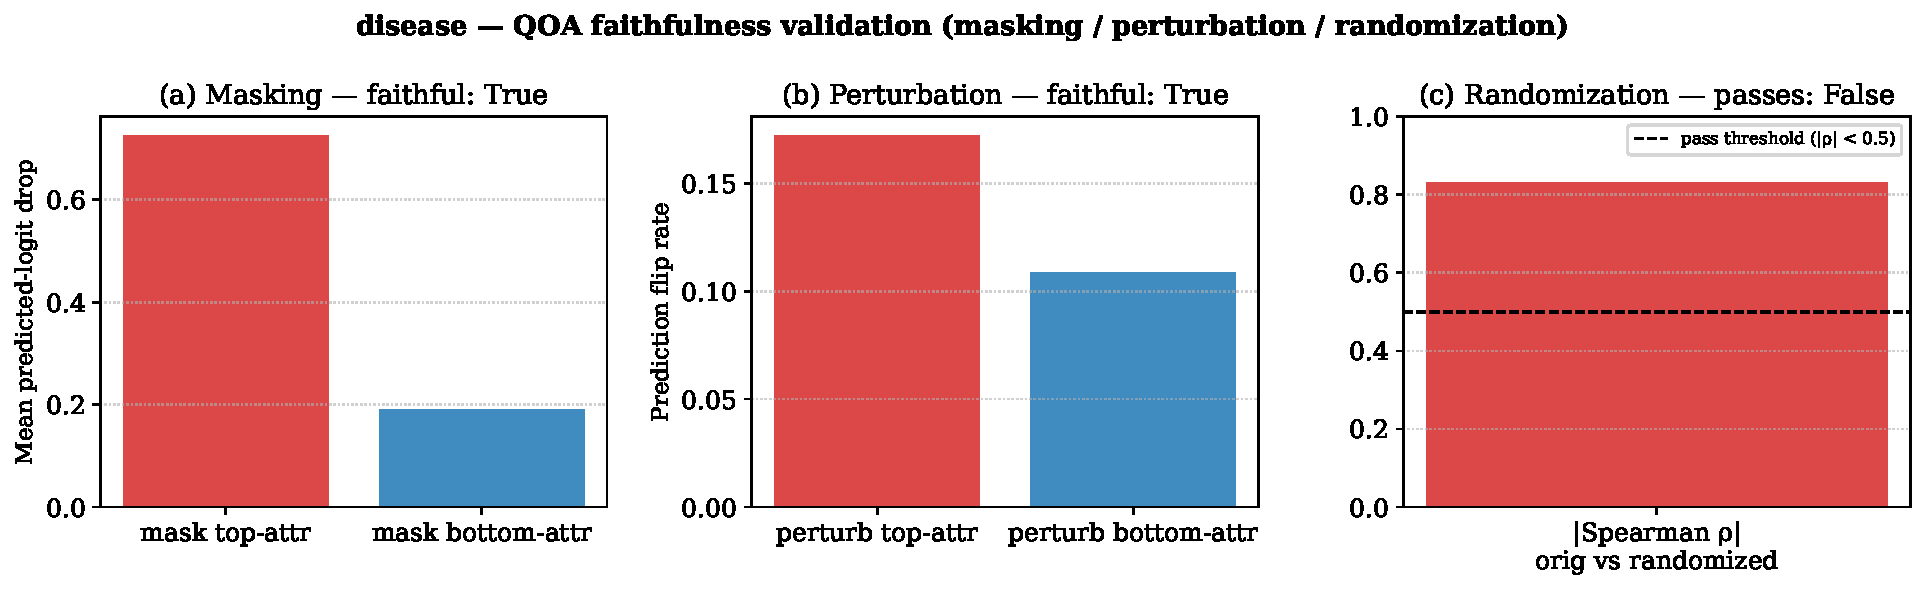
\includegraphics[width=0.49\textwidth]{figs/disease_xai_02_qoa_faithfulness.pdf}
\caption{QOA faithfulness harness, one panel per dataset (pilot models): masking logit-drops (top vs.\ bottom observable), perturbation flip rates (top vs.\ bottom), and the randomization Spearman $\rho$ against its $0.5$ threshold. Disease fails the randomization check only.}
\label{fig:faithfulness}
\end{figure}

We acknowledge the out-of-distribution critique of masking-style fidelity metrics \cite{ginxeval2023}: zeroed observables are off-manifold inputs. The randomization check is immune to this critique, which is why the harness requires all three verdicts rather than any one.

The broader XAI suite (Appendix~\ref{app:xai}) ports the conference version's five methods to the multi-dataset setting: integrated gradients on input features \cite{sundararajan2017ig}; QOA class$\times$observable heatmaps; Poincar\'e-disk visualization of the geo branch (2-D PCA of the tangent output, exp-mapped at learned curvature); gradient-attributed per-node quantum contribution ratio $r_Q$; and exact branch-level Shapley values \cite{shapley1953,lundberg2017shap} ($2^B$ coalitions over branches --- exact, unlike sampled KernelSHAP, and aligned with the leave-branch-out ground truth of H4).

\section{Discussion}\label{sec:discussion}

\paragraph{Why frozen $\ge$ trained is the expected result, in hindsight} Three independent lines converge. Barren-plateau theory predicts poor trainability of variational parameters even in small circuits when gradients are noisy and loss surfaces flat \cite{larocca2025barren}. The no-free-lunch result for untrained circuits \cite{herbert2023nfl} establishes that random circuits are not, on average, handicapped as feature maps. And Sect.~\ref{sec:failure}'s regime analysis shows the angle embedding confines the circuit to a small neighborhood of the identity, where its trainable parameters have little leverage but their gradients still inject noise into shared layers --- the network learns \emph{around} a fixed random projection faster than it can learn \emph{through} a moving one. The practical corollary for hybrid design: if a quantum branch is included, freezing it is the stronger default, and any claim that training the circuit helps should be required to beat that default under paired statistics.

\paragraph{Scope of the frozen-circuit claim} H5 is a statement about training a small circuit (4 qubits, depth 2, 24 variational parameters) \emph{behind a learned compressor that confines the embedding to a near-identity regime} --- the regime Sect.~\ref{sec:failure} measures on every dataset in this suite. Two scope limits follow. First, nothing here bounds larger circuits or richer embeddings; the claim is that under the design choices typical of current hybrid GNNs (small circuit, learned compression of sparse features), freezing wins or ties. Second, the regime itself is a candidate confounder: if the embedding used the full angle range, training might matter. We therefore added a post-freeze, explicitly exploratory control (disclosed in the preregistration amendment log): an \texttt{angle\_norm} variant that standardizes the compressed pre-activations so the embedding spans the full $\pm\pi$ range, re-running the frozen-vs-trained pair on Cora. The ordering not only persists --- it amplifies: under the full-range embedding the frozen circuit beats the trained one by $+11.8$ points on average, in 10/10 seeds (one-sided $p=0.001$), while both variants degrade and destabilize relative to the default embedding (trained $0.430\pm0.163$, frozen $0.548\pm0.160$). The near-identity regime therefore explains why training the circuit has little \emph{leverage}, not why it hurts; giving the circuit more leverage makes training it strictly worse. H5 is not an artifact of the embedding regime, and its scope is not narrowed by it.

\paragraph{What component accounting buys} Every headline in this paper is a difference between two configuration swaps. The protocol's cost is linear in the number of controls; its benefit is that claims become falsifiable at the component level. We suggest reviewers of hybrid QML papers request, at minimum: a frozen-parameter control for any trained quantum module, a parameter-matched classical surrogate, and per-branch gradient telemetry.

\paragraph{Limitations} All quantum execution is exact statevector simulation; finite-shot and hardware-noise behavior are preregistered follow-ups, and nothing here speaks to hardware readiness. Effect sizes shrank from pilot to confirmatory on nearly every comparison (H5 Cora $d$: $1.85 \to 0.87$; softmax mean gap: $10.4 \to 4.0$ n.s.; pooled H1 $p$: $0.004 \to 0.040$) --- the expected signature of selecting hypotheses on the population that suggested them, and the reason the two populations are kept disjoint; we treat the confirmatory numbers as the paper's claims and the pilot as context. With the registered family complete, no primary hypothesis survives family-wise correction at $\alpha=0.05$ (closest: H5 on Cora, Holm $p=0.056$ in the primary family; $0.074$ within the four-dataset H5 family). Four datasets support the pooled geometry analysis only weakly (Spearman over four points); the $\delta$-trend rejection is robust in sign but not in magnitude. The auxiliary-weight repair on Citeseer selected a grid-edge value ($2.0$), and the tuning budget, though equal-shaped across models, was necessarily modest. Finally, NEMA-Q's absolute accuracy trails tuned classical baselines on every standard benchmark --- this paper quantifies and explains that deficit rather than claiming advantage.

\section{Conclusion}\label{sec:conclusion}

Component accounting turns a hybrid model from a monolithic claim into an auditable ledger. Applied to NEMA-Q, the ledger reads: the hyperbolic encoder pays for itself (though not for the reason the literature gives), the fusion scaffold has a measurable and repairable failure mode but its gates are not attribution devices (H4 falsified), and the variational quantum circuit --- the component the architecture is named for --- contributes most when it is not trained at all. We offer the protocol, the instrumentation, and the preregistered-null discipline as the paper's primary contribution, and the frozen-circuit finding as its cautionary headline.

\backmatter

\bmhead{Data availability}
All datasets are public (Planetoid \cite{yang2016planetoid}; Disease from the HGCN repository \cite{chami2019hgcn}). Code, configuration files, run manifests, and the preregistration document are available at \url{https://github.com/Mahadi5577/Nema-Q} (preregistration frozen at commit \texttt{4605c73}; archived DOI to be minted at submission).

\bmhead{Author contributions}
MD Nurol Amin: Conceptualization, Methodology, Software, Investigation, Formal analysis, Writing --- original draft, Writing --- review \& editing.

\bmhead{Conflict of interest}
The author declares no competing interests.

\bmhead{Funding}
No external funding.

\begin{appendices}

\section{Parameter counts}\label{app:params}
Per-branch parameter counts on Cora (from run manifests): total $216{,}799$; hyperbolic branch $100{,}097$; quantum branch $6{,}080$ (of which $|\theta|=24$ circuit weights); classical bypass $95{,}936$. The parameter-matched surrogate replaces the circuit with an MLP matched to the quantum branch's count at 15\% tolerance, asserted by \texttt{tests/test\_param\_match.py}. Full per-seed tables are generated from the released manifests.

\section{EDA and \texorpdfstring{$\delta$}{delta} estimation}\label{app:eda}
Full exploratory data analysis (degree distributions, class balance, feature density, $\delta$ estimation detail) is reproducible from the released repository (\texttt{experiments/figures/eda}); Table~\ref{tab:datasets} summarizes the statistics used in the paper.

\section{Tuning grids and locked recipes}\label{app:tuning}
Default recipe: lr $0.01$, weight decay $5\times10^{-4}$, dropout $0.5$, aux weight $0.3$ (annealed), patience 100, epochs 500. Deviations (validation-selected, equal budget shape per dataset): Citeseer NEMA-Q/E/R --- lr $0.005$, aux $2.0$, gate bias $-4$; Disease GCN --- lr $0.05$, wd $5\times10^{-4}$, dropout $0.5$; Disease GAT --- lr $0.05$, wd $5\times10^{-5}$, dropout $0.5$; Disease HGCN --- lr $0.05$, wd $5\times10^{-5}$, dropout $0.2$; Disease NEMA-Q/E/R --- lr $0.05$, aux $0.3$, gate bias $-2$; all Disease configurations use patience 200. Sweep traces are preserved in the released notebook; the locked recipes are the committed yaml configs at the frozen commit.

\section{XAI suite figures}\label{app:xai}
The five-method XAI suite (integrated gradients, QOA heatmaps, Poincar\'e-disk visualization, quantum contribution ratio $r_Q$, exact branch Shapley) is generated per dataset by the released \texttt{analysis/xai.py}; figures for all four datasets accompany the repository.

\section{Preregistration}\label{app:prereg}
The full preregistration document (hypotheses, falsifiers, statistical protocol, locked recipes, dated amendment log) is frozen at repository commit \texttt{4605c73} as \texttt{experiments/PREREGISTRATION.md}.

\end{appendices}

\bibliography{sn-bibliography}

\end{document}
